\documentclass[12pt, a4paper]{ctexart}

% 页面与排版设置
\usepackage[margin=2.54cm]{geometry}
\usepackage{amsmath, amssymb}
\usepackage{booktabs}
\usepackage{graphicx}
\usepackage{float}
\usepackage{color}
\usepackage{xcolor}
\usepackage{array} 
\usepackage[colorlinks=true, linkcolor=black, urlcolor=blue, citecolor=black]{hyperref}
\usepackage{enumitem}           % 支持 enumerate 的 label= 参数

% 全局容差设置，彻底修复 Underfull / Overfull \hbox 警告
\setlength{\emergencystretch}{5em}
\tolerance=10000

% ---------- 字体与伪粗体设置 ----------
\usepackage{fontspec}
\setmainfont{Times New Roman} % 英文要求使用 Times New Roman

% 解决 macOS 字体找不到粗体产生的警告
\xeCJKsetup{AutoFakeBold=true}
\setCJKmainfont[AutoFakeBold=true]{Songti SC}      % 宋体
\setCJKsansfont[AutoFakeBold=true]{Heiti SC}       % 黑体
\setCJKmonofont[AutoFakeBold=true]{STFangsong}     % 仿宋

% ==========================================
% 全局中文标题样式设置 (严格遵循作业要求的“第X部分”格式)
% ==========================================
\ctexset{
    section = {
        format = \centering\zihao{3}\heiti, % 1级标题：黑体3号字居中
        name = {第,部分},   
        aftername = {：},                   % 冒号分隔，例如：第一部分：从辐射光到数字
        number = \chinese{section},         
    },
    subsection = {
        format = \raggedright\zihao{-3}\heiti, % 2级标题：黑体小3号字左对齐
        name = {},                       
        number = \arabic{section}.\arabic{subsection}, % 阿拉伯数字编号，如：1.1
    },
    subsubsection = {
        format = \raggedright\zihao{4}\heiti, % 3级标题：黑体4号字左对齐
        name = {},
        number = \arabic{section}.\arabic{subsection}.\arabic{subsubsection}, % 阿拉伯数字编号，如：1.1.1
    }
}

% 修复目录中 section 级别没有点点点的问题，包括摘要
\makeatletter
\renewcommand{\l@section}{\@dottedtocline{1}{0em}{1.5em}}
\makeatother

% 页眉页脚设置 (删除上方标题和页码，改为右下方)
\usepackage{fancyhdr}
\pagestyle{fancy}
\fancyhf{} % 清空所有的页眉和页脚
\renewcommand{\headrulewidth}{0pt} % 删除页眉的横线
\rfoot{\thepage} % 将页码放置在右下角

% 兼容 ctextart 自动调用 plain 样式的特殊页面（如目录首页）
\fancypagestyle{plain}{
    \fancyhf{}
    \renewcommand{\headrulewidth}{0pt}
    \rfoot{\thepage}
}

% ---------- 自定义上标引用命令 ----------
\newcommand{\scite}[1]{\textsuperscript{[#1]}}

\begin{document}

% ==========================================
% 自定义封面页
% ==========================================
\begin{titlepage}
\begin{center}
    ~\\[10.5pt]
    \textbf{\songti\zihao{1}  北京电影学院课程作业}
    ~\\[10.5pt] ~\\[10.5pt] ~\\[10.5pt] ~\\[10.5pt]

    {\zihao{2}\bfseries 数字影像显示再现全链路\\与前沿显示技术研究专题报告}
    
    ~\\[10.5pt] ~\\[10.5pt] ~\\[10.5pt] ~\\[10.5pt]
    ~\\[10.5pt] ~\\[10.5pt] ~\\[10.5pt] ~\\[10.5pt]
    ~\\[10.5pt] 
    
    \begin{tabular}{>{\heiti\fontsize{16pt}{16pt}\selectfont}r>{\kaishu\fontsize{16pt}{16pt}\bfseries\selectfont}l}
        作　　者：    &   祝庆\\[4pt]
        院　　系：    &   智能影像工程学院\\[4pt]
        专　　业：    &   影视技术\\[4pt]
        教学层次：    &   本科生\\[4pt]
        年　　级：    &   2023 级\\[4pt]
        学　　号：    &   231112014\\[4pt]
        指导教师：    &   顾晓娟 \hspace{0.5em} 鲁梦河\\[4pt]
        成　　绩：    &   \\[4pt]
        日　　期：    &   2026 年 5 月\\[4pt]
    \end{tabular}

\end{center}
\end{titlepage}

% ==========================================
% 前置部分（使用罗马数字页码：Ⅰ, Ⅱ, Ⅲ...）
% ==========================================
\newpage
\pagenumbering{Roman} % 设置页码为大写罗马数字并从1开始

% ==========================================
% 中文摘要（单独一页）
% ==========================================
\phantomsection
\addcontentsline{toc}{section}{中文摘要} % 将中文摘要手动加入目录
\begin{center}
    {\heiti\zihao{3} 内容摘要} 
\end{center}
\vspace{1em}
{\fangsong\zihao{-4} % 内容用小4号仿宋体字
\setlength{\parindent}{2em} % 起首空两格
本报告系统梳理了数字影像从“数字代码”重构为“物理光子”的完整显示链路。报告首先从底层解码与色彩空间转换切入，深入剖析了色域映射中“裁剪”与“压缩”的博弈，并通俗地解析了显示驱动微电路（DDIC）的物理工作机制；随后，横向对比了 Mini-LED、OLED 与 Micro-LED 三大主流硬件架构，揭示了其物理特性对高动态范围（HDR）内容呈现的深远影响。针对当前广色域屏幕普及带来的同色异谱现象，报告探讨了极窄带光源对传统 CIE 1931 色度学的严重挑战及业界的代偿方案。在核心的 HDR 理论环节，文章解构了 Gamma、PQ 与 HLG 在感知心理学上的非线性逻辑，并深度剖析了动态元数据（如 Dolby Vision 与 Gain Map）如何颠覆传统的色调映射范式。最后，报告对比了专业监视器与消费旗舰手机在色彩校准哲学上的根本分歧，并前瞻性地研究了智能像素驱动（Pixel-level AI）如何利用边缘算力重塑未来的显示生态。全文不仅追求学术推理的严谨，更辅以大量生活化类比，旨在为数字影像的学术研究与教学提供兼具深度与可读性的参考读物。\par
}

\vfill
% 关键词用4号黑体字，不超过5个以空格区隔
\noindent {\heiti\zihao{4} 关键词：数字影像\quad 色域映射\quad 高动态范围(HDR)\quad 同色异谱\quad Pixel-level AI}

% ==========================================
% 英文摘要（单独一页）
% ==========================================
\newpage
\phantomsection
\addcontentsline{toc}{section}{Abstract} % 将英文摘要手动加入目录
\begin{center}
    {\zihao{3}\textbf{Abstract}} 
\end{center}
\vspace{1em}
{\zihao{-4} % 内容用小4号 Times New Roman
\setlength{\parindent}{2em}
This report systematically outlines the complete display pipeline of digital imaging, reconstructing "digital code" back into "physical photons." It begins with bottom-level decoding and Color Space Conversion (CSC), analyzing the trade-offs between "clipping" and "compression" in Gamut Mapping, while intuitively explaining the physical mechanism of Display Driver ICs (DDIC). Subsequently, it compares the hardware architectures of Mini-LED, OLED, and Micro-LED, revealing how their physical characteristics profoundly impact the presentation of High Dynamic Range (HDR) content. Addressing the metameric failure caused by modern wide-gamut screens, the report explores the severe challenges narrowband light sources pose to traditional CIE 1931 colorimetry and the industry's compensatory solutions. In the core HDR theory section, the article deconstructs the perceptual non-linear logic of Gamma, PQ, and HLG, deeply analyzing how dynamic metadata (such as Dolby Vision and Gain Map) subverts traditional tone-mapping paradigms. Finally, the report contrasts the fundamental philosophical differences in color calibration between professional monitors and flagship consumer smartphones, and prospectively studies how Pixel-level AI utilizes edge computing to reshape the future display ecosystem. Balancing academic rigor with intuitive analogies, this report serves as an accessible and comprehensive reference for digital imaging education and research.\par
}

\vfill
% 英文关键词用4号 Times New Roman，排印在本页下端
\noindent {\zihao{4}\textbf{Key words:}\quad Digital Imaging\quad Gamut Mapping\quad HDR\quad Metamerism\quad Pixel-level AI}

% ==========================================
% 目录
% ==========================================
\newpage
\phantomsection
\addcontentsline{toc}{section}{目录} 
\renewcommand{\contentsname}{\centering\heiti\zihao{3} 目\quad 录}
\tableofcontents


% ==========================================
% 正文开始（使用阿拉伯数字页码，且格式为 01, 02...）
% ==========================================
\newpage
\pagenumbering{arabic} % 页码切换回阿拉伯数字并重置为1
\renewcommand{\thepage}{\ifnum\value{page}<10 0\arabic{page}\else\arabic{page}\fi} % 小于10前面补0

\newpage
\section{显示再现全链路——从数字到光}

数字影像的显示再现是一个高度复杂的多学科交叉过程，涵盖了数字信号处理、色彩科学、微电子学以及光学物理等领域\scite{1}。如果把摄像机的拍摄比作“把风景打包进数字集装箱”，那么显示再现就是“在观众的视网膜前重新搭建这片风景”\scite{2}。从一串冰冷的数字码值转化为最终刺激视网膜的物理光子，整个链路需要经历极为严密的解构、重绘与物理激发\scite{3}。在当今异构显示设备共存的生态中，如何确保创作者的视觉意图在不同的硬件载体上得到忠实还原，是显示全链路技术的核心命题。

\subsection{信号解码与色彩空间转换 (CSC)}

显示设备接收到的数字影像信号（如 HEVC、AVC 编码的视频流或 JPEG、HEIC 等图像文件）通常处于特定的编码色彩空间与非线性压缩状态中\scite{4}。为了节省极其昂贵的传输带宽，工程师不会直接传输 R、G、B 三个完整的通道，而是采用“色度子采样（Chroma Subsampling）”技术，将图像拆分为负责亮度的 Y 通道和负责色彩的 Cb、Cr 通道（如 4:2:0 格式）\scite{5}。这就像是一幅素描草稿（Y）加上几块大面积的色块（CbCr），利用人眼对亮度敏感、对色彩分辨率迟钝的生理漏洞，成功骗过视觉系统。

显示再现的第一步，便是\textbf{信号解码与色彩空间转换（Color Space Conversion, CSC）}\scite{6}。解码器首先将 YCbCr 进行逆向矩阵运算，恢复出非线性的 R'G'B' 信号\scite{7}。然而，这仅仅是信号处理的开端。在现代多设备生态中，源视频的色彩空间（如好莱坞常用的 DCI-P3 或广播级的 Rec.2020）往往与目标显示器面板的原生物理发光能力不重合。这就需要进行精确的色彩“翻译”。

翻译的过程需要一个“中转站”\scite{8}。系统首先必须通过电光转换函数（EOTF）剥离非线性压缩，将其变成场景的绝对线性光（Linear RGB）。这一步至关重要，因为所有的色彩矩阵相乘只有在光度线性的空间下才具有物理意义。接着，线性 RGB 会通过一个 $3 \times 3$ 的变换矩阵，被映射到一个与任何设备都无关的绝对连接空间（Profile Connection Space, PCS），最常用的即是 CIE 1931 XYZ 空间\scite{9}。在这个空间里，如果源内容是在标准 6500K 白光下调色的，而目标手机屏幕当前被 True Tone 传感器校准在 5500K，系统会执行色度适应转换（Chromatic Adaptation Transform, CAT，通常使用 Bradford 矩阵）。最后，再通过一个针对目标面板定制的逆向矩阵，生成目标显示器独有的物理驱动 RGB 码值。

\subsection{色域映射的核心逻辑：裁剪与压缩}

当数字影像内容的色域超出了目标显示器的物理显示能力时，系统必须依靠色域映射（Gamut Mapping）算法来处理超出色域（Out-of-Gamut）的颜色\scite{10}。色域映射不仅涉及二维的色度坐标平面（即色相和饱和度），更是一个包含亮度（Luminance）在内的三维色量（Color Volume）处理过程。这就好比要把一张巨大的宽幅风景画，硬塞进一个相对较小的标准相框里\scite{11}。系统通常有两种核心处理哲学：

\begin{enumerate}
    \item \textbf{裁剪（Clipping / Absolute Colorimetric Intent）}\scite{12}：这种逻辑的原则是“死守绝对准确”。相框能装下的部分（色域内颜色）保持绝对原样，数值上一丝一毫都不改变。而装不下的边缘部分，则被无情地“一刀切断”，强行贴在相框的边框上（映射到目标色域边界上距离最近的可显示颜色）。
    \begin{itemize}
        \item \textit{代价}：导致高饱和度或极高亮度区域（如霓虹灯、爆炸的高光中心）失去层级梯度\scite{13}。比如画面中有一个从中心向外逐渐变淡的红苹果，如果最红的中心超出了屏幕能力，裁剪算法会把这部分全部变成同一种“最红”，导致苹果看起来像贴了一块纯色的死板红色塑料片，这在专业术语中称为色带断层（Banding）\scite{14}。
    \end{itemize}
    \item \textbf{压缩（Compression / Perceptual Intent）}\scite{15}：这种逻辑的原则是“保持相对关系”。为了把宽幅画作塞进小相框，算法会把整张源色域体积按比例非线性地整体收缩到较小的目标色域内。这意味着即使是原本在显示器物理能力范围内的颜色，也会被轻微改变（通常是降低一点点饱和度），以此为那些极端鲜艳的颜色“腾出平滑过渡的空间”。
    \begin{itemize}
        \item \textit{优势}：人眼其实很难记住绝对的颜色代码，但对颜色之间的“明暗对比和渐变过渡”极其敏感。非线性压缩深度契合了人眼的感知特性，保留了苹果圆润的反光梯度和立体感，是目前 HDR 到 SDR 色调映射过程中最核心的底层逻辑基础\scite{16, 17}。
    \end{itemize}
\end{enumerate}

\subsection{显示驱动电路：从数字量到光量子的跨越}

经过上述色彩空间转换与色域映射后生成的最终目标数字 RGB 码值，需要通过精密的显示驱动电路转化为控制物理像素发光的电信号。该过程依赖于显示器背板（Backplane）电路与显示驱动芯片（Display Driver IC, DDIC）的紧密协同，实现了从布尔逻辑到模拟物理量的跨越。

对于现代有源矩阵（Active Matrix）显示器，每个像素下方均配备了由薄膜晶体管（TFT）和存储电容（$C_{storage}$）组成的微电路控制网格。现今高端显示器广泛采用了 LTPS（低温多晶硅）或 IGZO（铟镓锌氧化物）作为 TFT 沟道材料，以获得极高的电子迁移率，从而缩小晶体管体积，提高像素开口率。DDIC 内部的核心部件是数模转换器（DAC），它将数字信号解码，并转化为对应的模拟电压信号（Source Voltage, 即 $V_{Data}$）。

\begin{itemize}
    \item \textbf{在 LCD 面板中（电压驱动 PAM）}：液晶单元本身不发光，而是通过改变偏振态来充当背光光阀。当显示周期的选通信号打开开关 TFT 时，DAC 输出的模拟电压 $V_{Data}$ 会对存储电容进行充电。电容维持的该电压施加在液晶层上，使得液晶分子产生特定角度的扭转，从而精确控制背光透过的光子数量，实现不同灰阶的再现（脉冲幅度调制 PAM）\scite{18, 19}。
    \item \textbf{在 OLED 等自发光面板中（电流与 PWM 驱动）}：OLED 像素自己就是微型光源。经典的 OLED 像素驱动电路采用 2T1C（两个 TFT 加上一个电容）甚至是更复杂的 7T1C 补偿结构。驱动 TFT 根据其栅源电压差（$V_{gs}$）来控制注入 OLED 的电流（$I_{OLED}$）。然而，当应对极低灰阶的精准控制时，单纯依赖降低模拟电流会导致有机发光材料的波长漂移（Color Shift）以及亮度的非均匀性（偏绿或偏红）。因此，高端智能手机与显示器引入了\textbf{高频脉宽调制（PWM）调光}技术。PWM 极其聪明：它不改变流经二极管的峰值电流大小，而是保持电流恒定，通过在一个极其微小的刷新周期内高速切换像素的“开”与“关”状态来实现调光。它利用人眼的视觉暂留效应，通过改变“开启”状态的时间占比（占空比）来实现感知亮度的变化\scite{20}。占空比越宽，感知越亮\scite{21}。PWM 彻底解决了低亮度下的偏色问题，但为了防止人眼疲劳，现代旗舰手机通常需要将 PWM 频率提升至 1440Hz、2160Hz 甚至 3840Hz 以上，才能有效规避隐形频闪带来的神经损害。
\end{itemize}

\newpage
\section{HDR 硬件原理、分类及分析}

为了支撑高动态范围（HDR）内容中严苛的高峰值亮度与极低黑位要求，传统全局背光的 LCD 就像一个“同亮同暗的大灯箱”，完全无法胜任。业界由此衍生出革命性的硬件架构。然而要理解这些革命，我们必须先从最基础、最经典的液晶显示技术（LCD）讲起——它是所有现代显示技术的基础\scite{22}。

\textit{【注：本部分关于各主流显示技术（LCD、Mini-LED、OLED、QLED 以及 Micro-LED）的硬件原理配图、核心内部拆解结构图及部分底层物理原理解析，均参考自 Bilibili 知名科普视频（BV1Me4y1k72b），特此声明并致谢该视频提供的直观视觉拆解资料以辅助学术理论的论述。】}

\begin{figure}[H]
    \centering
    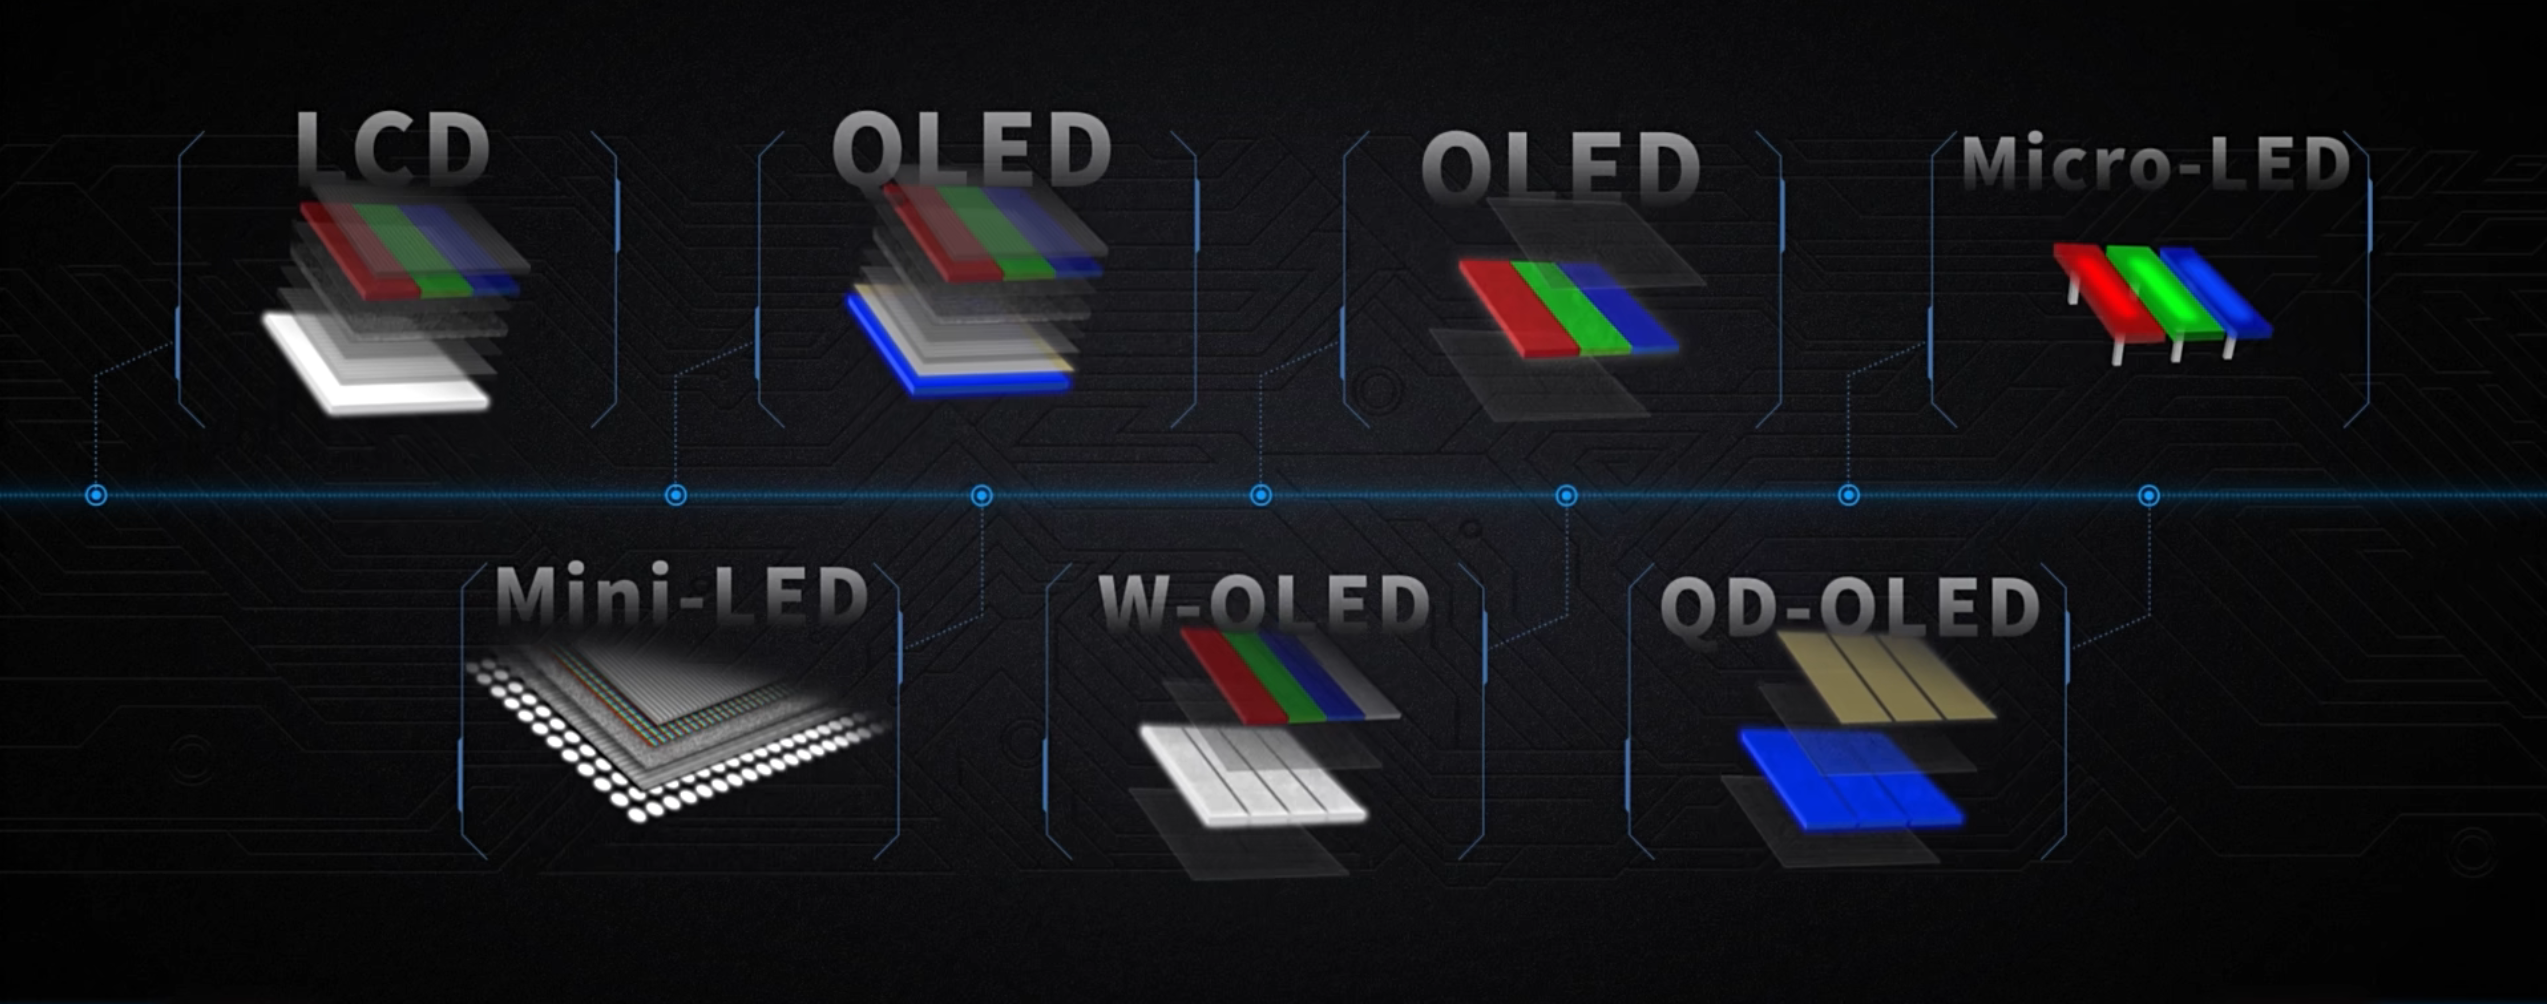
\includegraphics[width=0.9\textwidth]{显示技术进化分类图谱.png}
    \caption{显示技术进化分类图谱（源自 BV1Me4y1k72b）。横向梳理了从传统 LCD 到 OLED、QD-OLED、Mini-LED 及 Micro-LED 等主流技术路线，标出各自的技术分支与演进关系。}
    \label{fig:tech_evolution}
\end{figure}

图 \ref{fig:tech_evolution} 给出了一个宏观的路线图，展示了本部分将要讨论的几大技术阵营在整个显示进化树中的位置。从经典的液晶体系到自发光的有机与无机路线，每一次分化都是为了解决前一个方案在对比度、亮度或寿命上的短板。

\subsection{从 LCD 出发：液晶显示的基本原理}

液晶显示器（LCD）本身并不发光。它像一扇精心设计的“百叶窗”，需要背后有一个大灯箱（背光）才能让人看见画面。这扇“百叶窗”由数百万个微小的液晶分子组成，它们夹在两片玻璃基板之间。液晶分子的特殊之处在于：它们像小针一样，平时是杂乱排列的，但当施加电压时，它们会整齐地扭转方向。扭转的角度决定了它们能“挡住”多少背后灯箱的光线。

\begin{figure}[H]
    \centering
    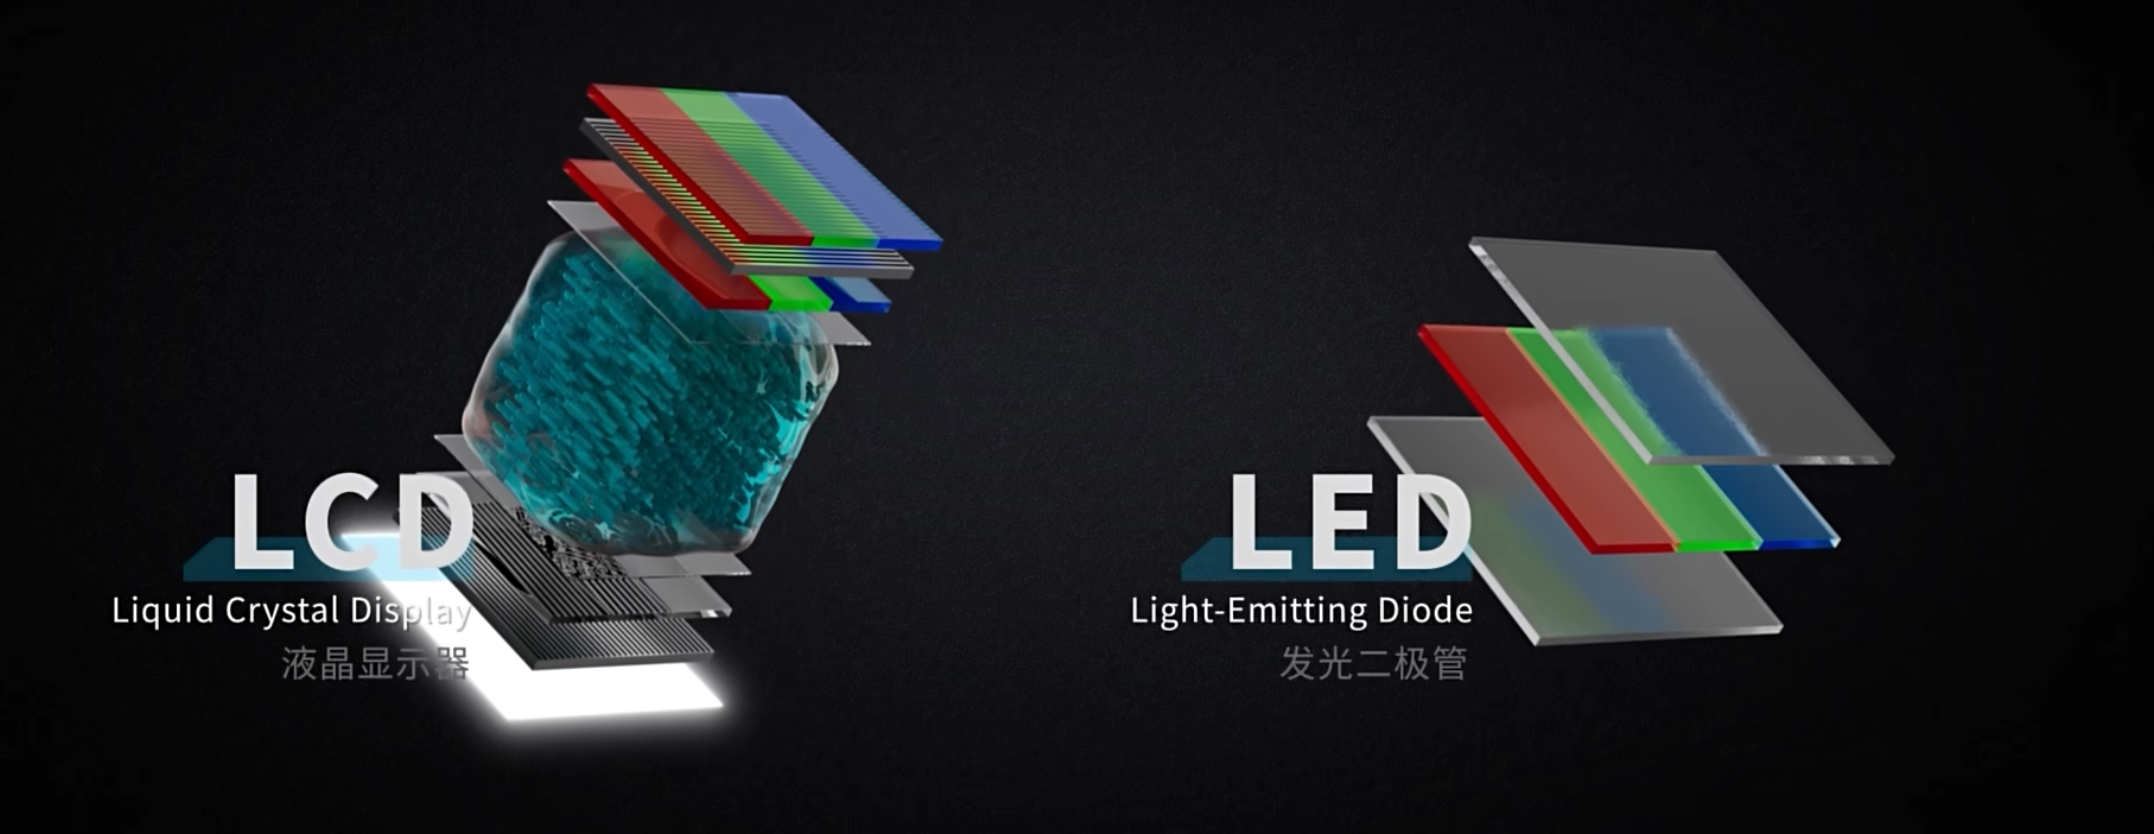
\includegraphics[width=0.85\textwidth]{LCD与LED结构对比.png}
    \caption{LCD 与 LED（指 LED 背光 LCD）结构的立体拆解对比（源自 BV1Me4y1k72b）。两图均标注了液态晶体层与背光层的基本组成，右图强调背光已从 CCFL 灯管升级为 LED 光源。}
    \label{fig:lcd_led_structure}
\end{figure}

图 \ref{fig:lcd_led_structure} 将传统 CCFL 背光方案与后来的 LED 背光方案并列拆解，让我们可以直观理解“灯箱”的进化路径。而在像素层面，图 \ref{fig:lcd_oled_cross} 展示了 LCD 与 OLED 的横截面差异。

\begin{figure}[H]
    \centering
    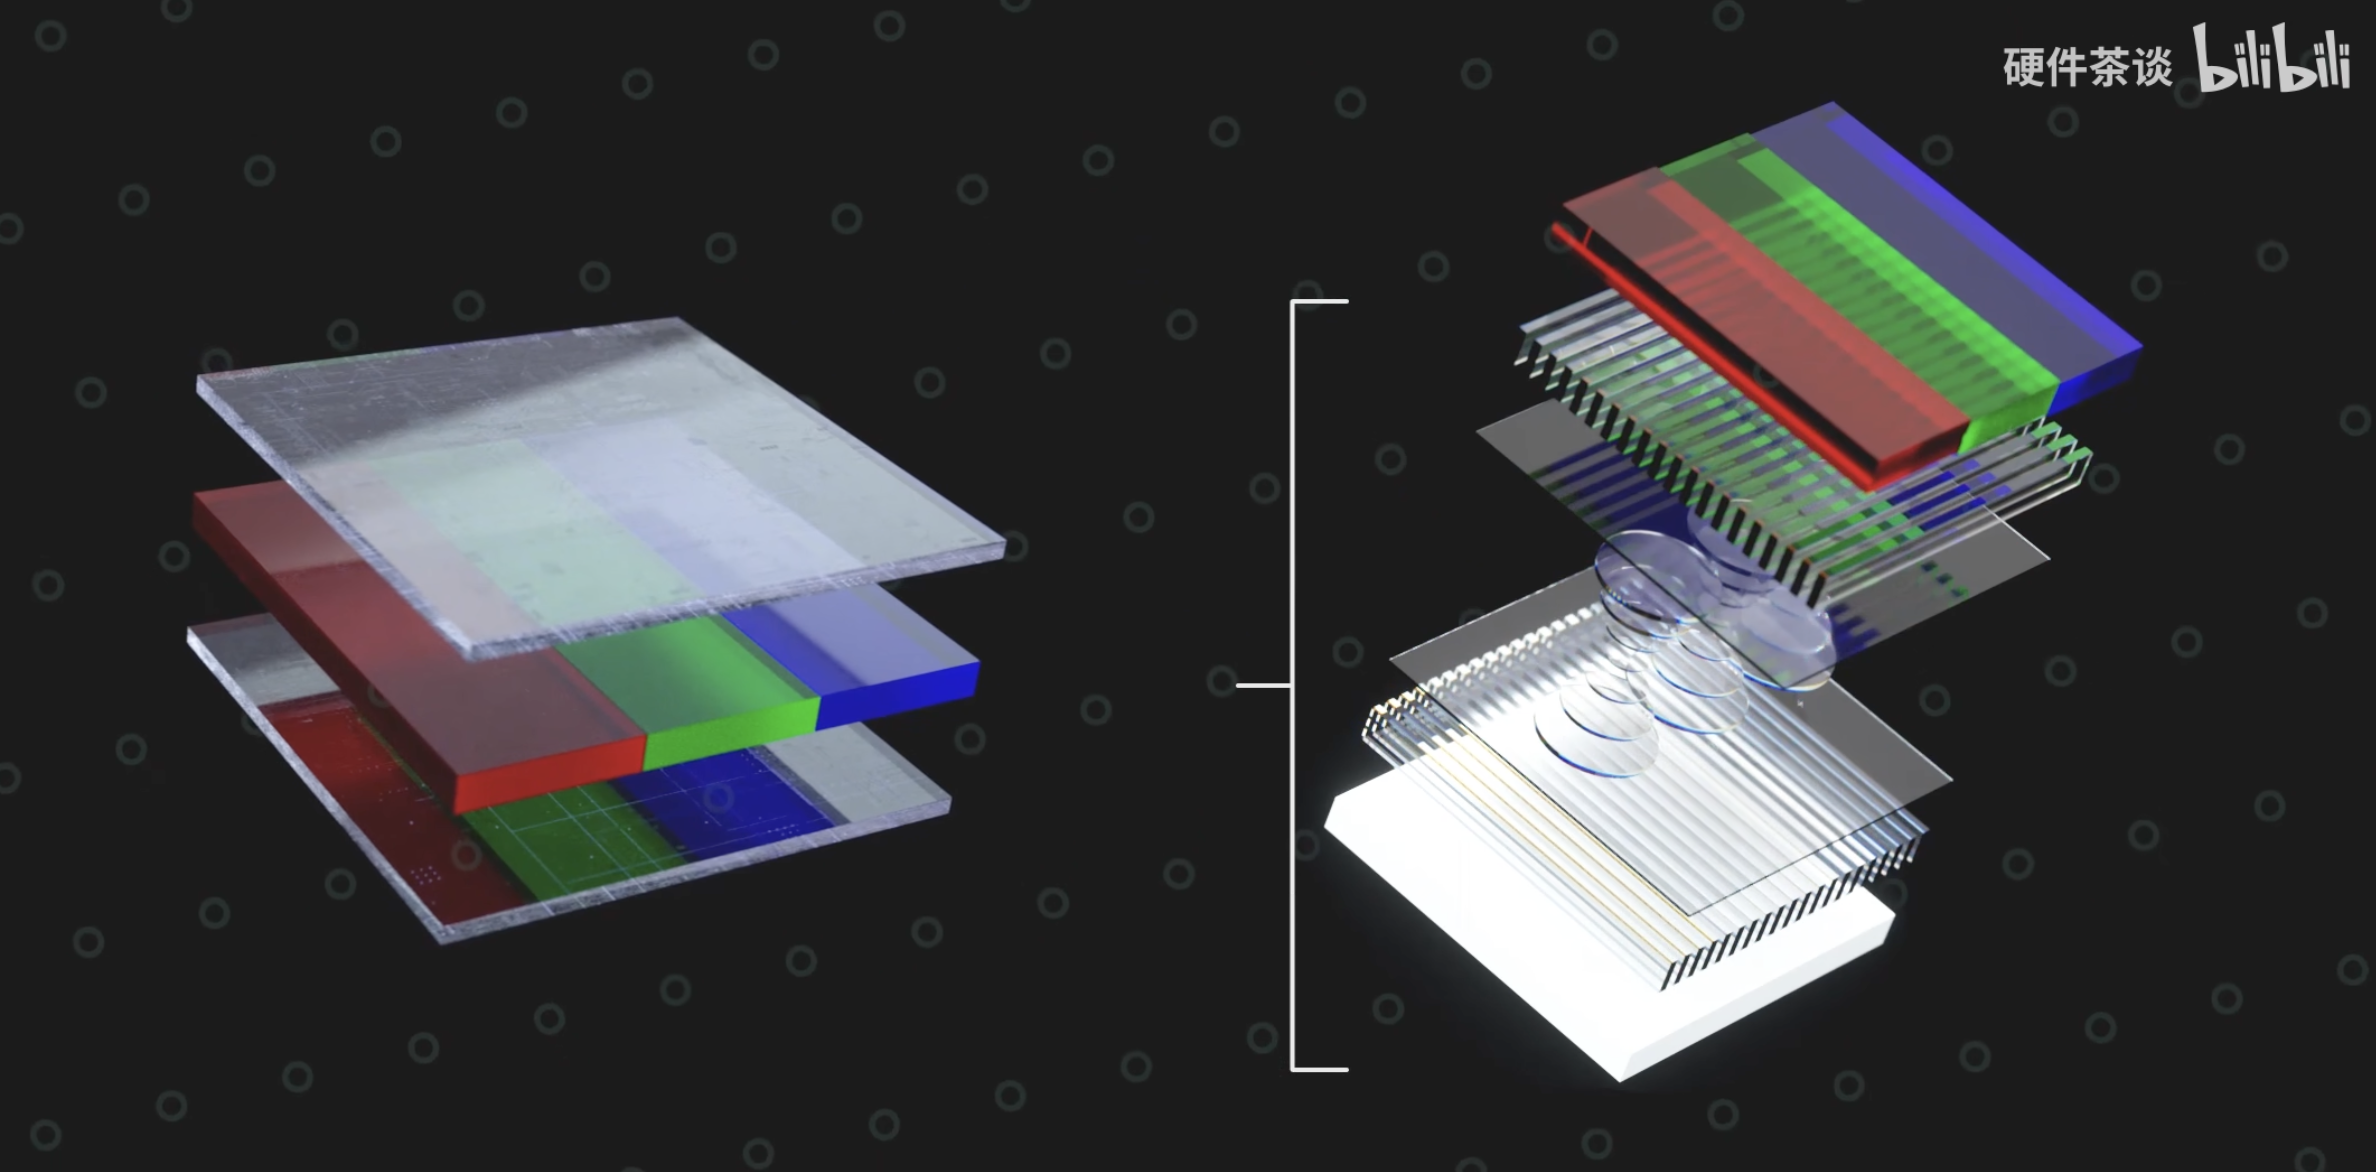
\includegraphics[width=0.8\textwidth]{OLED与LCD成像原理对比.png}
    \caption{典型 TFT-LCD 像素结构与 OLED 自发光像素结构对比示意图（源自 BV1Me4y1k72b）。右半部分：LCD 依赖背光与液晶层，包含偏光片、彩色滤光片、TFT 阵列；左半部分：OLED 每个 RGB 子像素独立发光，无需背光。}
    \label{fig:lcd_oled_cross}
\end{figure}

请观察图 \ref{fig:lcd_oled_cross} 的右半部分，那是传统 LCD 像素的“横截面”。从上往下看：
\begin{itemize}
    \item 最上层是\textbf{偏光片}，它像一副只允许垂直光波通过的栅栏。
    \item 接着是\textbf{玻璃基板}，上面刻有\textbf{彩色滤光片}（红、绿、蓝三原色的小块）。每个像素又被分割成三个子像素。
    \item 中间是\textbf{液晶层}——就是那扇会扭转的百叶窗。
    \item 再往下是\textbf{另一片玻璃基板}，上面布满了\textbf{薄膜晶体管（TFT）} 阵列。每一个子像素都由一个独立的 TFT 开关控制，TFT 就像给每个小窗户配了一个专属的“电动马达”。
    \item 最下面是\textbf{背光模块}——那个提供恒定白色光的大灯箱。
\end{itemize}

当 TFT 给液晶分子施加电压时，液晶分子会扭转，让背光的光线穿过偏光片和彩色滤光片，最终射入人眼。电压越高，扭转角度越大，透过的光越多，该子像素就越亮。这就是\textbf{电压驱动调光（PAM）} 的基本原理。然而，传统 LCD 的背光是全局的，导致其对比度通常只有 1000:1 左右，黑位总是呈现出泛灰的视觉观感。

\subsection{从 CCFL 到 Mini-LED：背光的进化与光晕的诞生}

为了解决 LCD 黑位不黑的痛点，工程师开始把背光分割成几十个、甚至几千个独立的“灯区”。这就是 \textbf{Mini-LED} 诞生的逻辑。Mini-LED 的灯珠只有几百微米大小，一块电视上可以塞进数千个独立的灯区。这就像从“用手电筒照亮整个房间”进化到“用几千个微型探照灯分别照亮每一小块地板”。

\begin{figure}[H]
    \centering
    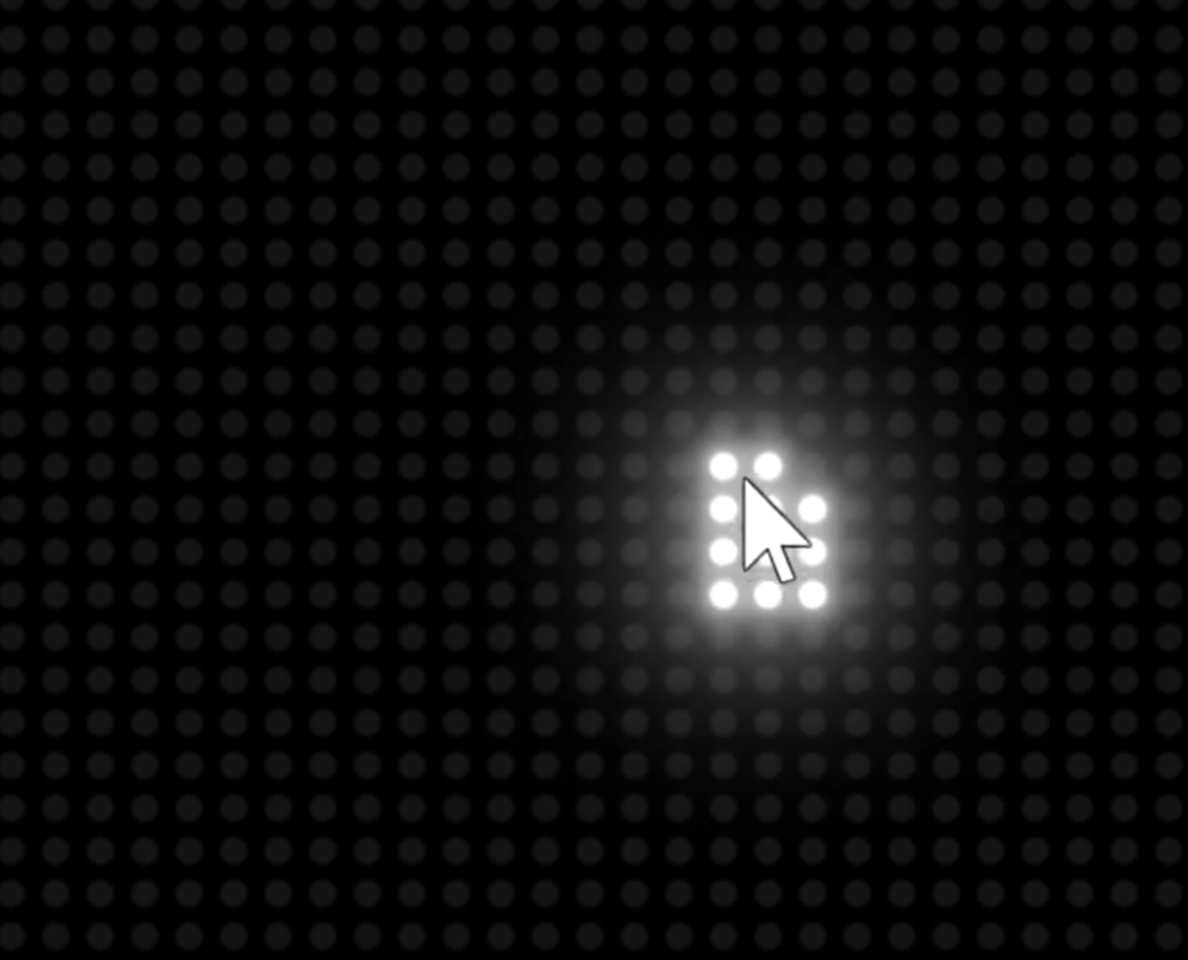
\includegraphics[width=0.7\textwidth]{Mini-LED-局部背光演示.png}
    \caption{Mini-LED 局部背光点阵示意（源自 BV1Me4y1k72b）。背光层中密布着大量独立可控的发光单元，每一个小方块代表一个调光分区，可在极暗场景下单独点亮或关闭，实现分区背光。}
    \label{fig:mini_led_demo}
\end{figure}

图 \ref{fig:mini_led_demo} 直观呈现了 Mini-LED 背光层中密集排列的调光点阵。正是这些独立可控的微型发光单元，使 LCD 首次获得了接近像素级的明暗控制能力。Mini-LED 擅长释放恐怖的峰值亮度（2000–4000 尼特），但不可避免地会带来\textbf{光晕（Blooming）}现象。由于一个灯区往往覆盖几十个液晶像素，在点亮暗背景中的孤立亮点时，光线会不可避免地溢出到四周的纯黑像素中。

\begin{figure}[H]
    \centering
    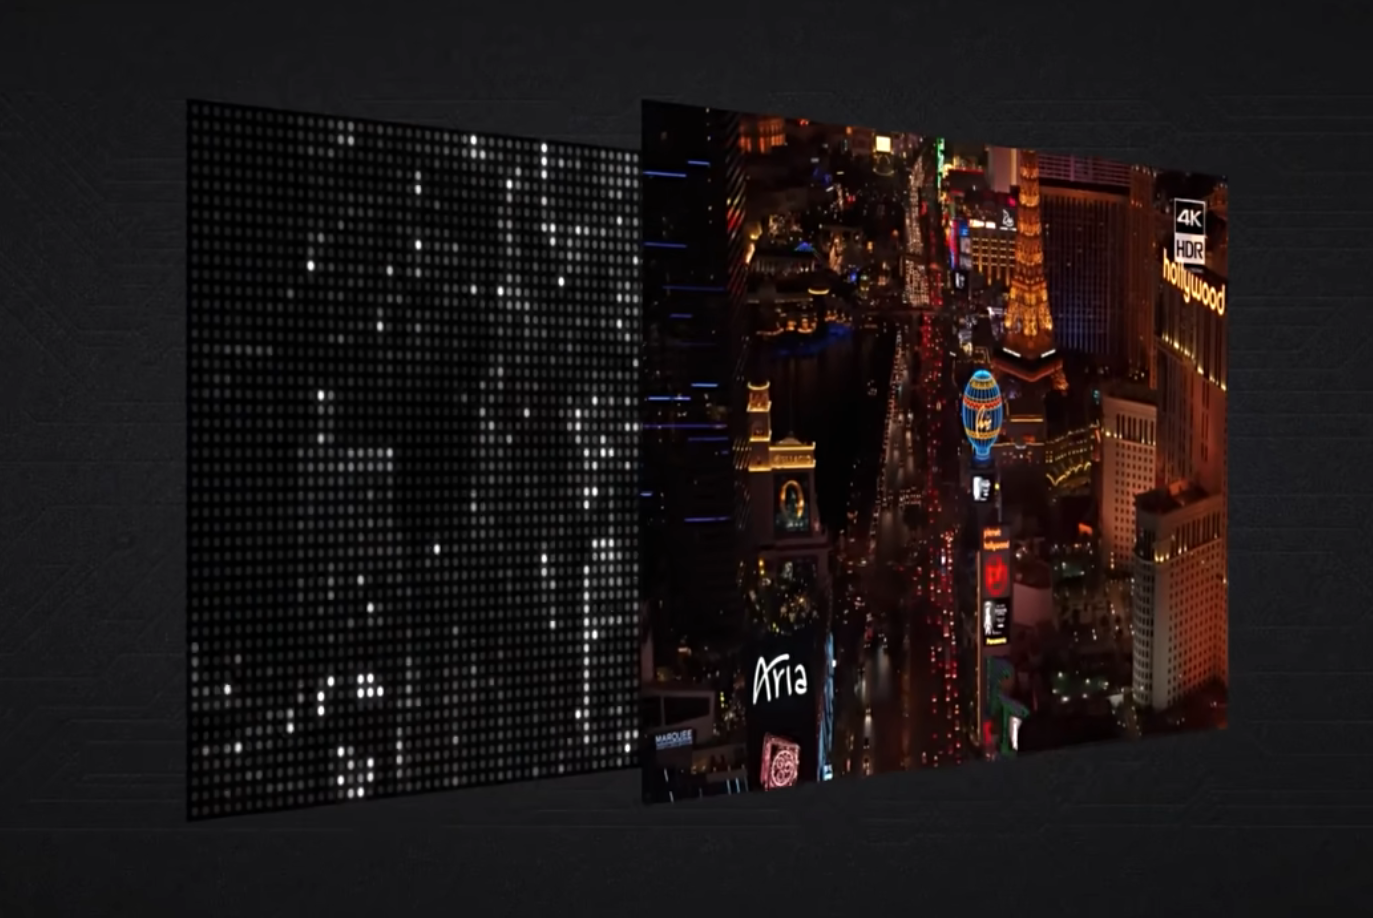
\includegraphics[width=0.9\textwidth]{背光点阵与实拍画面对比.png}
    \caption{背光点阵与实拍画面的对应关系（源自 BV1Me4y1k72b）。左图为 Mini-LED 背光层点阵的明暗分布，右图为最终合成的画面。}
    \label{fig:backlight_vs_image}
\end{figure}

\begin{figure}[H]
    \centering
    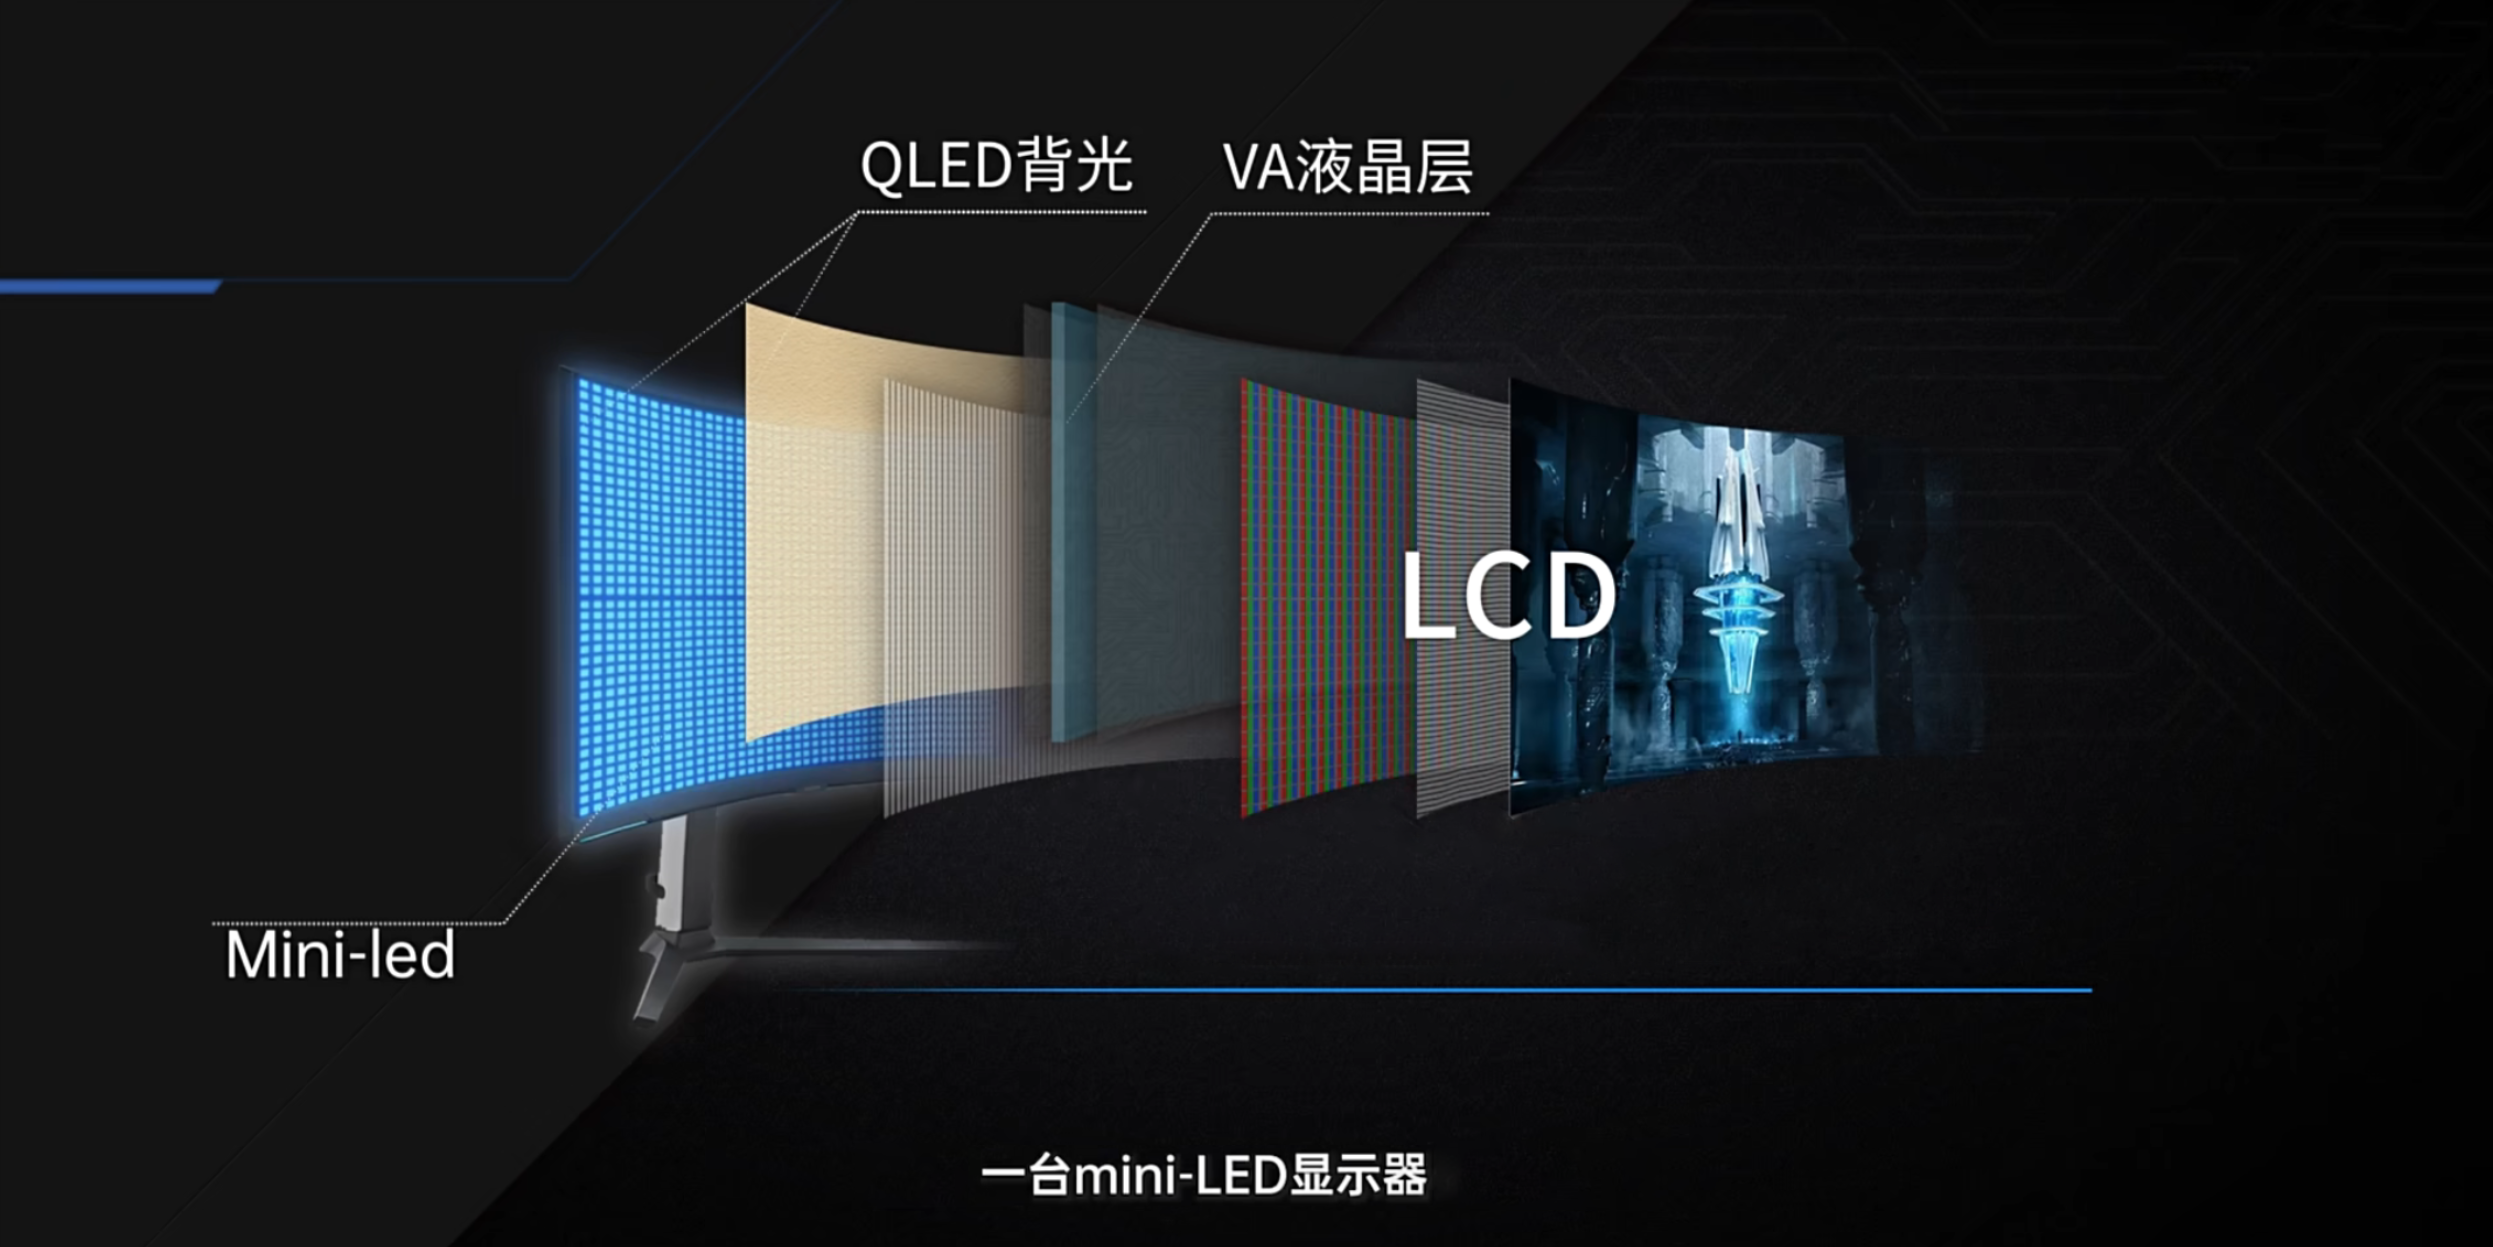
\includegraphics[width=0.85\textwidth]{Mini-LED显示器多层结构图.png}
    \caption{一台以 Mini-LED 为背光的曲面显示器多层结构拆解（源自 BV1Me4y1k72b）。图中标出了 Mini-LED 背光阵列、QLED 膜以及 VA 液晶面板等复合堆叠层级。}
    \label{fig:mini_led_layer}
\end{figure}

\subsection{OLED：自发光像素的优势与挑战}

另一种完全不同的结构是\textbf{自发光像素}。这里的核心变化是：\textbf{没有背光，没有液晶层，每个像素自己就是一只微小的灯泡}。这正是 OLED（有机发光二极管）的工作原理\scite{20}。

\begin{figure}[H]
    \centering
    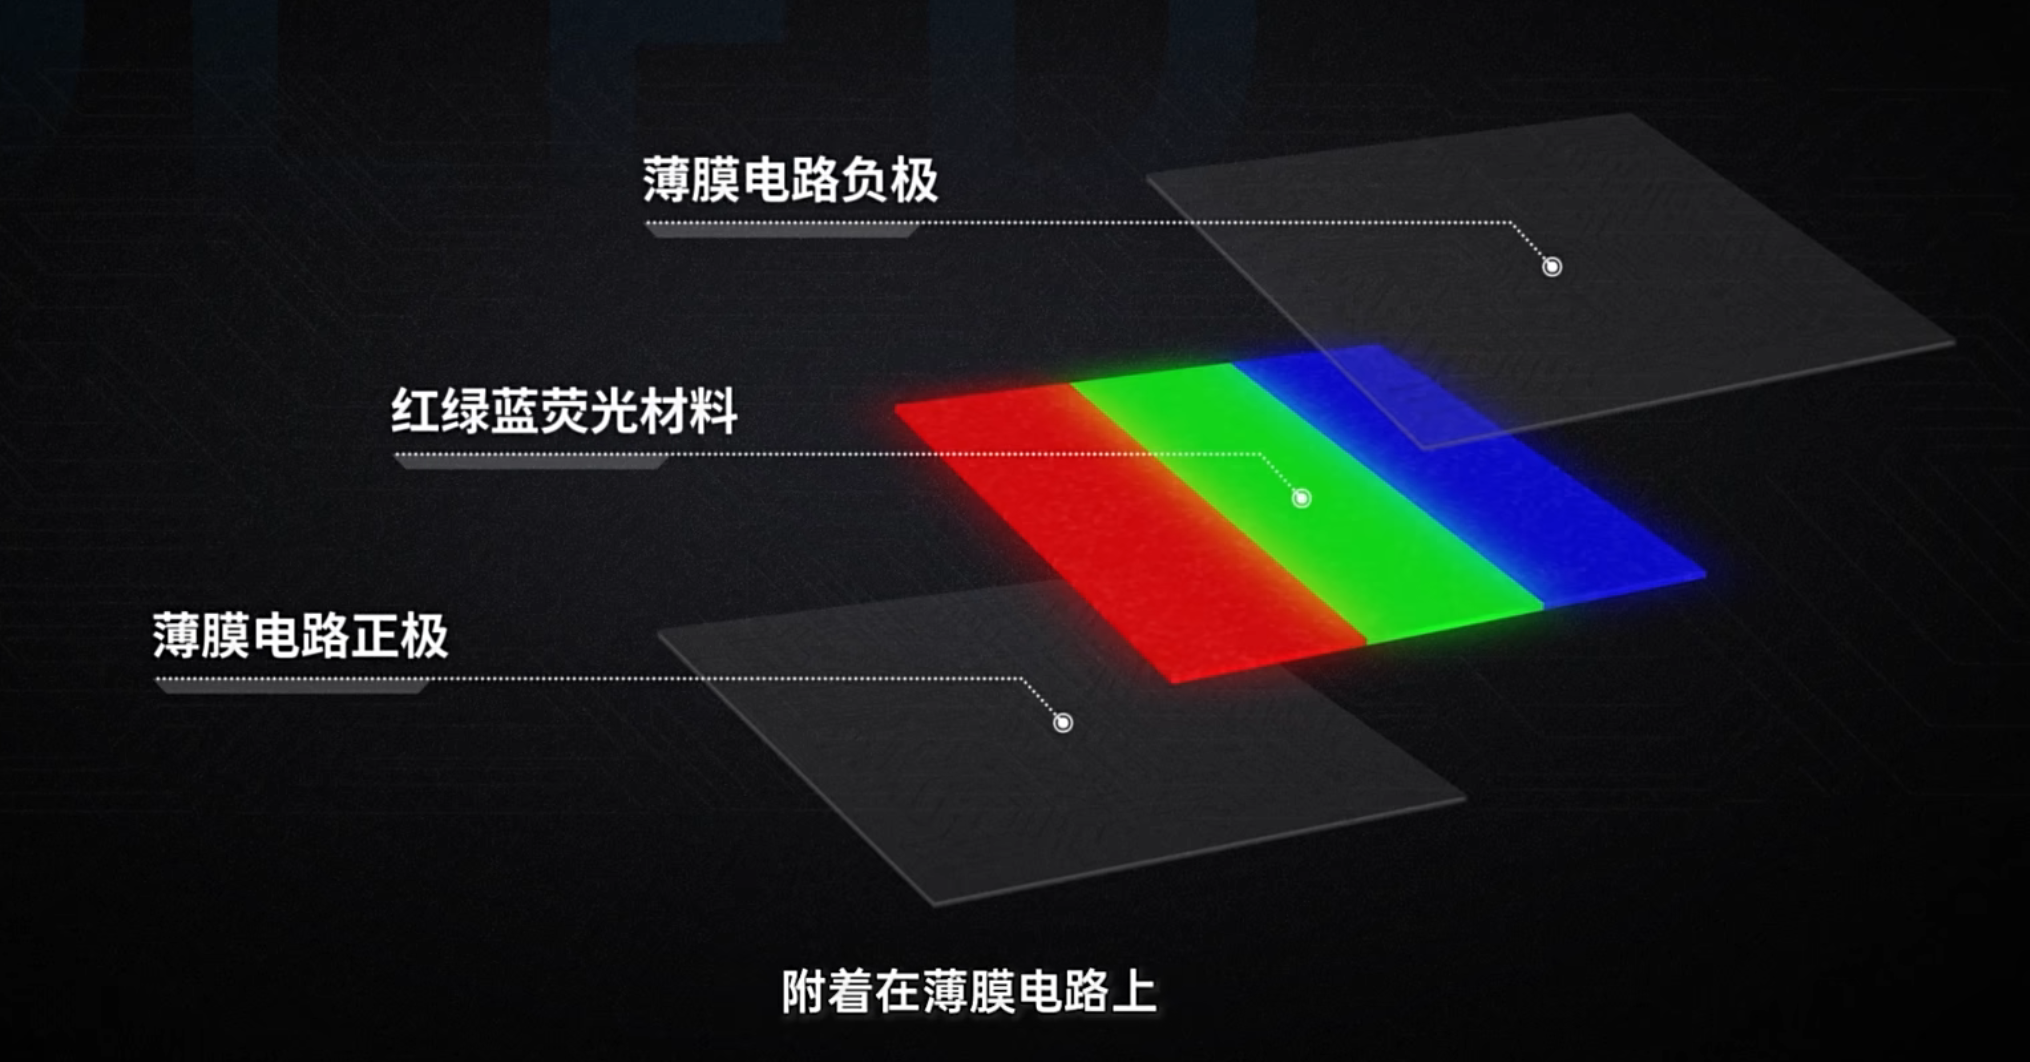
\includegraphics[width=0.65\textwidth]{OLED基本结构层.png}
    \caption{OLED 典型三层结构示意（源自 BV1Me4y1k72b）。中间为红、绿、蓝有机荧光发光材料，上下分别为薄膜电路的正极与负极，构成一个完整的自发光像素单元。}
    \label{fig:oled_structure}
\end{figure}

OLED 直接堆叠在电极和 TFT 驱动电路之上，通电即亮。它拥有\textbf{绝对纯黑}（不发光的像素物理断电，亮度为真正的 0 尼特）、\textbf{无限对比度}与\textbf{极快的响应速度}。但 OLED 存在三个硬伤：烧屏风险（有机材料老化）、自动亮度限制器（ABL 强制压制大面积高光以保护面板）以及低灰阶下的发光效率偏色现象。

\subsection{Micro-LED：终极的理想与现实}

Micro-LED 同样采用自发光架构，但其发光材料替换成了\textbf{微米级的无机半导体晶体}。它融合了 OLED 的像素级纯黑控光与 Mini-LED 的恐怖无机高光，峰值亮度可轻松突破 10,000 尼特，且毫无烧屏与 ABL 的烦恼。Micro-LED 被公认为“显示技术的终极神殿”，但目前受限于巨量转移（Mass Transfer）工艺的良率极低，导致成本极其昂贵，难以普及。

\subsection{窄带显示硬件：QLED、量子点技术与多色/单色激光投影}

除了在对比度和亮度维度进行突破，为了追求极致的色彩纯度与 DCI-P3 甚至 Rec.2020 广色域，业界还衍生出了以量子点（Quantum Dot）和激光为代表的窄带发光硬件结构。

\begin{figure}[H]
    \centering
    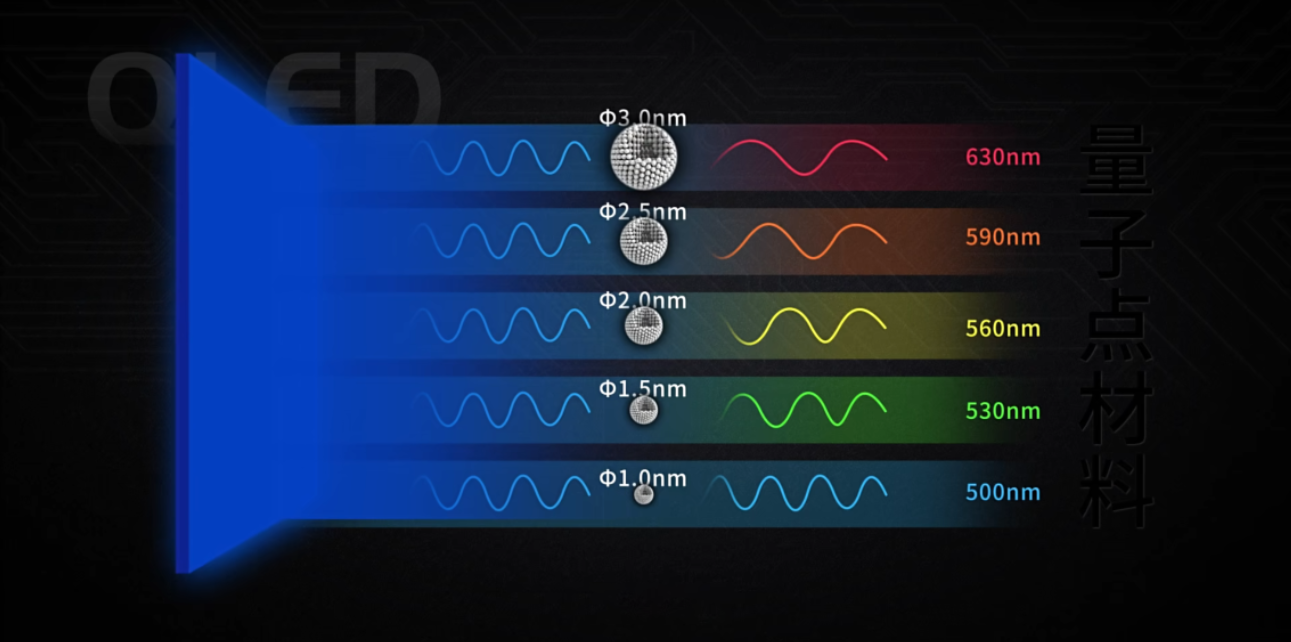
\includegraphics[width=0.9\textwidth]{量子点材料发光原理.png}
    \caption{量子点材料发光原理（源自 BV1Me4y1k72b）。量子点受蓝光激发后重新发射波长精确的光，直径越小波长越短（偏蓝），直径越大波长越长（偏红），是实现窄带纯色发射的关键技术。}
    \label{fig:qled_principle}
\end{figure}

图 \ref{fig:qled_principle} 揭示了窄带光源背后的核心物理机制：量子点（QD）是一种纳米级别的半导体晶体。当受到高能短波光（如纯蓝光 LED）激发时，量子点能够吸收能量并重新发射出波长极其精确的窄带光。最神奇的物理特性在于，仅仅通过控制这些纳米晶体的物理直径大小，就能精准决定其发射光的波长：直径较小的量子点发出偏蓝的短波光，而直径较大的量子点则发出偏红的长波光。这种通过“物理尺寸”来切割“光学波长”的机制，造就了目前显示面板界最纯净的基色。

\begin{figure}[H]
    \centering
    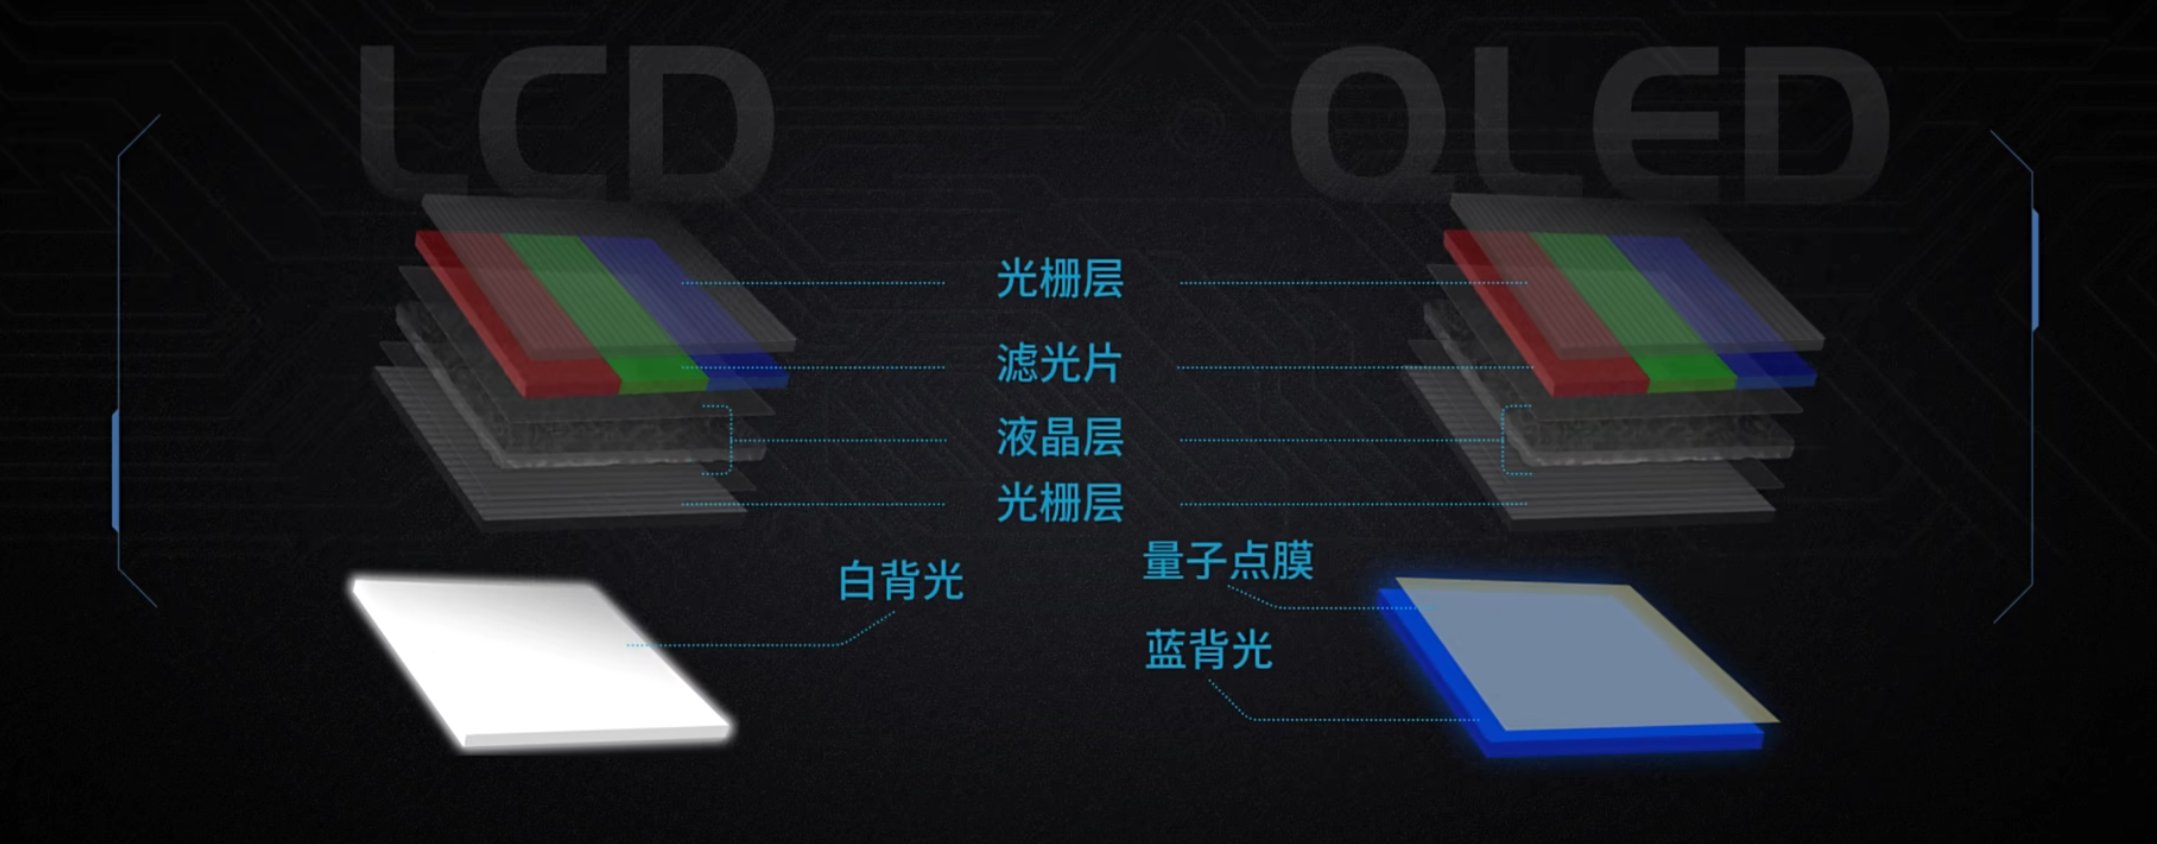
\includegraphics[width=0.9\textwidth]{LCD与QLED详细结构对比.png}
    \caption{普通 LCD（白背光）与 QLED（蓝背光 + 量子点膜）的详细结构对比（源自 BV1Me4y1k72b）。传统白背光光谱杂乱，而 QLED 通过量子点膜（QDEF）将蓝光转换为光谱极度尖锐的红、绿光。}
    \label{fig:lcd_vs_qled}
\end{figure}

图 \ref{fig:lcd_vs_qled} 详细对比了普通 LCD 与 QLED（量子点液晶电视）的结构差异。传统 LCD 依赖涂有荧光粉的白色 LED 背光，其光谱宽泛且杂乱。而 QLED 方案则直接使用高能量的纯蓝光 LED 作为背光层，并在背光与液晶层之间插入了一层布满红色和绿色量子点的量子点增强膜（QDEF）。由于发射出的红光和绿光频带极其狭窄，色彩不仅异常纯粹，还大幅提升了整个显示系统的发光效率。该技术同样被应用于现今高端的 QD-OLED 面板中（使用蓝色 OLED 作为激发源）。

\paragraph{多色与单色激光投影：}
在巨幕影院与高端家用投影领域，激光显示技术代表了极致色域的另一种路径。单色激光投影（通常采用 ALPD 荧光激光技术）利用单束高能蓝光激光打在高速旋转的荧光色轮上激发产生红绿光，受限于荧光粉材料，其色纯度有上限。而真正的多色（三色 RGB）激光投影，则彻底抛弃了荧光粉，直接使用独立发射红、绿、蓝三种极窄波段的半导体激光器（Laser Diodes）进行混光。三色激光的发射光谱带宽往往不到 5nm，是目前唯一能够理论上达到 100\% Rec.2020 色域覆盖率的“终极光源”。然而，这种极其尖锐的光谱除了带来散斑（Speckle）问题外，还引爆了一个巨大的色彩科学隐患——同色异谱失败。

\subsection{上述主流硬件对 HDR 内容呈现的综合限制与促进}

理解了这些硬件原理后，我们就能深刻理解物理架构对数字 HDR 内容的最终呈现起到了怎样的决定性作用：

\begin{itemize}
    \item \textbf{Mini-LED 擅长高 APL（平均图像电平）的宏大亮度表达}：面对暴晒的沙漠等高亮全景，其无机背光可彻底释放压迫感；但在暗场星空等孤立亮点场景下，物理防区溢出的\textbf{光晕}会严重破坏沉浸感，迫使调色师有时不得不压抑星星的亮度以妥协硬件缺陷。
    \item \textbf{OLED 擅长微光纯净与深邃暗场}：像素级控光使得暗部细节完美无瑕；但受限于 \textbf{ABL（自动亮度限制器）}，大面积高光的突然爆发会被强制拉低，导致外景 HDR 冲击力断崖式下跌。
    \item \textbf{Micro-LED 剥离了双向限制}：融合了像素级纯黑和无机万尼特高光，是杜比视界 4000 nits 甚至 10000 nits 母版信号的不妥协容器。
    \item \textbf{QLED 与 三色激光投影 极大扩展了 HDR 的色量（Color Volume）边界}：HDR 不仅包含亮度，还包含极端的色彩体积。窄带光源物理上赋予了 HDR 内容在极高明度下依然保持极高饱和度（例如赛博朋克风格中耀眼的霓虹红、绿灯）的能力，这是传统滤光片 LCD 永远无法企及的色彩极限。
\end{itemize}

\newpage
\section{窄带显示对色度学与测量的挑战}

在第二部分中，我们探讨了 QLED（量子点技术）与三色激光投影等硬件，如何依靠发光光谱极其狭窄的发射器来追求覆盖 Rec.2020 的极致色彩饱和度。然而，这项物理上的突破却直接动摇了现代色彩管理和仪器测量的根基，引爆了一个潜伏了近 90 年的历史遗留炸弹——\textbf{同色异谱失败（Metameric Failure）}\scite{24}。

\subsection{同色异谱失败与人眼生理的“局部盲区”}

在传统显示工业中，无论是万元级的校准探头还是后期的色彩管理软件，其计算大脑中都内置了一套名叫 \textbf{CIE 1931 2° 标准观察者模型（Color Matching Functions, CMFs）} 的数学函数\scite{25}。这是 1930 年代科学家基于极其有限的光学实验建立起来的“人类视锥细胞平均敏感度响应曲线”。

“同色异谱”本是显示技术的物理根基：红绿蓝三种完全不同的物理光波，混合后恰好能刺激出特定的视锥细胞反应，令人眼产生“这是纯白光”的感知错觉。但致命问题在于，现代神经科学证明，CIE 1931 模型并不完美，它在极度深蓝（短波）和深红（长波）的波段，严重低估了人类视网膜的实际敏感度\scite{26}。

在宽带背光（如 CCFL 或常规 W-LED）时代，屏幕的光谱能量分布很宽，犹如钝刀，这一生理学误差被宽频带大面积掩盖了。但当 QLED、QD-OLED 和三色激光的极窄带光柱（带宽小于 5-10nm）刺向视网膜时，它们犹如手术刀般精准切中了 CIE 1931 模型误差最为严重的盲区\scite{27}。

结果灾难性地发生了：\textbf{高精度的校准色度计通过 CIE 1931 函数进行数学积分后，信誓旦旦地显示这台 QD-OLED 电视与旁边的传统 LCD 参考级监视器达到了绝对完美的 D65 白点匹配（色坐标分毫不差）；但调色师用肉眼一看，却发现 QD-OLED 严重偏黄绿或偏洋红}\scite{28}。仪器测量的数据与人类视网膜的主观感知在这里彻底断裂，这种因窄带光诱发的人眼视觉背离，就是同色异谱失败。此外，由于人眼晶状体老化黄变程度不同，导致不同年龄段的调色师盯着同一台激光电视，看到的偏色程度竟然也存在显著的个体生理差异。

\subsection{学术界与工业界的应对方案}

为了解决仪器数据与人类主观感知“打架”的尴尬局面，业界展开了从硬件测量到数学底层的自救：

\begin{enumerate}
    \item \textbf{引入替代观察者模型（CIE 170-2:2015）}\scite{30}：治本之法是抛弃 1930 年代的老旧残缺数据。基于现代神经视觉科学，国际照明委员会发布了全新的 CIE 2015 观察者模型。该模型精准重构了 L、M、S 视锥细胞的敏感度，甚至在数学上将人类晶状体随年龄增长发黄的生理特征参数化，引入了“年龄计算变量”。在使用 CIE 2015 模型重新计算后，仪器得到的数据终于能够和人眼在窄带屏幕上的主观所见保持高度统一。目前，诸如 Calman 等顶尖色彩软件已经内置了此模型供好莱坞机房调用。
    \item \textbf{高分辨率分光辐射度计（Spectroradiometer）的强制应用}：传统的廉价色度计依靠三个固定频宽的物理滤色片来模拟人眼，面对极度尖锐的窄带光时，光子极易从滤色片的感应波谷中“漏掉”，导致庞大误差。工业界现在被强制要求使用光学分辨率在 2nm 到 5nm 级别的超高精度分光辐射度计。这种设备抛弃了滤色片，直接用光栅将光线物理打散，捕捉每一纳米频率上的绝对光谱功率分布（SPD），再将原始数据交给软件用新模型进行数学积分。
    \item \textbf{显示校准偏移（Judd-Vos / White Point Offset）的工业骗局}：由于全球广播、影视工业标准（如 Rec.709/2020）均死死绑定了 CIE 1931，一夜之间更换底层算法将引发数字生态的全面瘫痪。因此，专业监视器大厂（如 Sony）发明了一个极其聪明但透着无奈的实用主义方案——\textbf{人为刻意测偏}。工程师找来一群专家，纯靠肉眼将新型窄带屏幕的白点调到和传统宽带基准屏幕“看起来一样”的舒适状态。此时用仪器一测，发现坐标实际上偏移到了 $x: 0.306, y: 0.322$。厂商随后在出厂写入芯片时，直接把这个错误的“偏移坐标”当作绝对目标锁定。这就是所谓的“用测量仪器的数学错误，来强行换取人眼生物感知的正确”。
\end{enumerate}

\newpage
\section{HDR显示技术深度解析}

高动态范围（HDR）不仅仅是拉高背光驱动电流那么简单，它是一场从数字传输协议、色调映射哲学到感知心理学的全链路重构。如果说前文提到的面板和量子点是汽车的物理发动机，那么下面将要剖析的传递函数（Transfer Functions）和动态元数据（Metadata）就是控制发光逻辑的终极变速箱系统\scite{31}。

\subsection{EOTF 与视觉非线性映射逻辑：Gamma、PQ 与 HLG 的底层解构}

传递函数构成了数字代码与物理光子之间的转化桥梁。其中，\textbf{EOTF（电光转换函数）} 负责把数字码值（如 0-1023）翻译为屏幕表面绝对的物理发光亮度（尼特）\scite{32}。为什么这种转换不能是一条 1 码值对应 1 尼特的简单直线？因为人类眼睛的对数感知特性决定了，我们在暗室中对 1 尼特的微光变化极其敏感，但在正午阳光下增加 100 尼特却几乎毫无察觉（韦伯-费希纳定律）\scite{34}。

\begin{itemize}
    \item \textbf{Gamma 曲线（SDR时代的霸主）}：最初是源于阴极射线管（CRT）物理缺陷的妥协，却阴差阳错地极其契合了人眼对暗部敏感的特征。但在亮度飙升至 1000 尼特乃至 10000 尼特的 HDR 时代，如果强行把 Gamma 曲线拉长，在高光区域会严重浪费数字比特，导致暗部由于缺乏编码空间而出现灾难性的色带断层（Banding）。
    \item \textbf{PQ (Perceptual Quantizer, SMPTE ST.2084) 的极致量化}：杜比实验室抛弃了 Gamma，基于人类对比度极其敏锐的极限模型研发了 PQ 曲线\scite{35}。杜比的测试确立了一个名为 \textbf{Barten Ramp（巴顿阈值）} 的人类视觉对比度分辨极限曲线。PQ 的伟大之处在于其极其精密的非线性数学设计：当使用 12-bit 深度的 PQ 曲线编码时，从 0.0001 尼特到极致的 10,000 尼特区间内，数字码值每一次微小的跳变步进，都严格保持在 Barten 阈值的下方！这意味着系统以绝对不浪费任何一个比特的最高效率，确保了人眼绝对看不出色带断层。即使降级使用 10-bit，PQ 曲线也仅仅是略微贴在巴顿阈值上方，在绝大多数场景中依然能保持平滑\scite{36, 37}。它是数字编码效率的数学奇迹。
    \item \textbf{HLG (Hybrid Log-Gamma, ARIB STD-B67) 的拼图式妥协}：由 BBC 与 NHK 开发的直播领域 HDR 标准。它的非线性曲线由两部分拼接而成：下半部分（暗部和中间调）使用传统的 Gamma 曲线以保持对老旧 SDR 电视的向后兼容；而在上半部分（极高亮度区），则依据 Weber 定律切换为对数（Logarithmic）曲线以剧烈压缩高光动态范围\scite{38, 39}。与 PQ 强绑定绝对物理亮度不同，HLG 呈现的是“相对光度”，无需元数据，画面峰值由电视本身的硬件极限决定，成为了广播电视实时转播的救星。
\end{itemize}

\subsection{OOTF 系统伽马的物理与心理学本质}

\textbf{OOTF（光光转换函数）} 描述的是“真实世界场景光”和“最终电视屏幕发射光”的整体宏观映射关系。从物理还原论来看，OOTF 似乎应该是一条斜率为 1 的完美直线（即 $OETF \otimes EOTF = 1$），但事实恰恰相反，\textbf{OOTF 绝对不能是线性的}。

这里隐藏着一个深度的生理学 Bug：\textbf{Bartleson-Breneman 效应}\scite{40}。该心理物理学效应揭示，当人类身处黑暗的环境（如熄灯的电影院、昏暗的客厅）观看明亮的显示屏时，视觉系统会发生强烈的适应性偏移，导致我们主观觉得画面原本正常的暗部变得发灰、对比度大幅下降。为了在“黑暗的心理预期”中补偿这种生理错觉，系统必须人为地引入一个大于 1 的系统伽马（System Gamma）。例如，在极暗环境中必须将整体伽马提高到 1.5 左右，在较暗客厅则设定在 1.2。

在 HLG 规范中，为了补偿不同亮度电视带来的主观错觉，其系统伽马 $\gamma$ 甚至被公式强制要求与电视的标称峰值亮度 $L_W$ 挂钩：$\gamma = 1.2 + 0.42 \log_{10}(L_W / 1000)$。由此可见，OOTF 的核心绝不是克隆物理光子，而是为了在不同观看环境下“欺骗”大脑，而施加的环境感知补偿与艺术渲染意图\scite{41}。

\textbf{探讨深度迷思：为什么 PQ (ST.2084) 刻意不定义对应的 OETF？}
在 ITU 等国际标准中，HLG 明确规定了 OETF，但 PQ 只有孤零零的显示端 EOTF。这是因为 PQ 被设计为一个\textbf{“显示端绝对参照物（Display-referred）”}。在影视工业中，无论前期的摄影师是用 ARRI 的 LogC 还是 Sony 的 S-Log 拍摄（这本身就是各种复杂的 OETF），调色师都会在后期机房内加上各种主观的对比度调节、风格化 LUT 及环境补偿（这构成了极其主观且无法用标准固化的 OOTF）。调色师最后渲染出的那个文件，就是希望屏幕实实在在要发光的物理指令包。既然影像系统遵循 $OETF = OOTF \otimes EOTF^{-1}$，且 PQ 被设定为了一个强制执行数字与物理尼特挂钩的终端尺子，再去反向规定源头必须用哪种标准 OETF，已经毫无工程意义\scite{42}。

\subsection{动态元数据处理与色调映射革命：HDR10、Dolby Vision、HDR10+ 与 Gain Map 的全面对比}

受限于多数消费级电视面板远无法达到杜比视界 4000 尼特甚至 10000 尼特的母版上限，必须通过算法将超高亮度的超限内容“压缩”回电视的物理极限，这一过程称为色调映射（Tone Mapping）。这就需要元数据（Metadata）出场了。

\textbf{1. HDR10（静态元数据的“以偏概全”）}：它在视频开头封装了诸如 MaxCLL（整部片子最亮的单个像素值）等静态数据。如果一部两小时的深沉暗调电影中，仅在最后一秒闪过一个 4000 尼特的爆炸高光，电视底层的处理器就会为了这短暂的瞬间，依据 4000 尼特的峰值参数强行压低那 1 小时 59 分钟的昏暗场景，导致整部电影的黑位和中间调沉闷无比，层次尽失。

\textbf{2. Dolby Vision 与 HDR10+（动态元数据的“实时微操”）}：为了对抗静态映射的弊端，杜比视界与三星牵头研发的 HDR10+（标准化为 \textbf{SMPTE ST 2094-40}）引入了革命性的动态元数据机制\scite{43, 44}。它们不再给一个毫无指导意义的静态全局极值，而是通过嵌入 JSON 格式的数据或 SEI 消息，以“逐场景（Scene-by-scene）”甚至“逐帧（Frame-by-frame）”的频率，实时刷新并将当前帧画面的真实直方图、最大亮度和平均亮度等详尽特征喂给电视的处理器。
当播放暗室低语的场景时，元数据告诉电视“这一帧最亮仅有 100 尼特，你可以彻底放宽映射曲线，充分拉升暗部纹理”；而当画面切到阳光下的雪地时，元数据瞬间下发指令收紧高光曲线，避免云层过曝死白。这种随着时间轴疯狂变化的动态微操，使得低峰值亮度的中端电视也能逼近高端母版的生动层次。

\textbf{3. Gain Map（增益图）：空间自适应的生态降维打击（ISO 21496-1）}
虽然动态元数据主宰了视频领域，但在跨设备分享极度碎片化的静态照片领域，HDR 的兼容性始终是灾难。基于最新国际标准 \textbf{ISO 21496-1} 确立的 \textbf{Gain Map（增益图）} 则打出了一套精妙绝伦的架构降维打击\scite{45, 46}。

Gain Map 抛弃了直接传输高亮绝对值的做法。它在底层容器中储存了一张经过极其完美调色、绝对安全且对比度柔和的传统 SDR 图像（Base Image）；同时，将高光区域亮度应该如何呈指数级翻倍的空间信息，编码成一张非常小巧的隐藏灰度图（即 Gain Map，增益图），作为元数据嵌入文件深处。
当这张照片被发到老旧的、不支持 HDR 的显示器或 App（如普通的网页或旧款手机）上时，系统读不懂增益图，于是干脆忽略它，直接显示出那张极其完美的 SDR 底图——保证了颜色绝不发灰。
而当照片流转到最新支持 HDR 的旗舰手机（如 iPhone 15 Pro 或最新安卓机皇）上时，渲染引擎检测到屏幕具备极高的硬件余量（Headroom），系统瞬间抽取这层隐藏的增益图，将其作为乘法器矩阵，逐个像素地叠加在 SDR 底图上。一瞬间，照片中的太阳光晕和霓虹灯招牌在屏幕上解锁了刺眼的高光效果。Gain Map 凭借极其优雅的“差值叠加数学模型”，使得同一个数字文件实现了跨越几十年代差硬件的绝对向后兼容，构筑了未来影像互联的底层基石。

\newpage
\section{前沿探索：显示校准与环境光自适应技术对比}

数字显示技术在不同的工业应用场景中，因其背负的使命不同，分化出截然相反的发展路径。其中，专业影视母版监视器与消费级高端智能手机在对待“色彩一致性与感知适配”这一命题上的理念分歧，构成了当代色彩科学最引人注目的悖论。以下表总结了它们在核心架构上的异同：

\begin{table}[H]
\centering
\caption{专业电影基准监视器与旗舰级智能手机设计哲学对比}
\begin{tabular}{@{} >{\raggedright\arraybackslash}p{2.5cm} >{\raggedright\arraybackslash}p{6.5cm} >{\raggedright\arraybackslash}p{6.5cm} @{}}
\toprule
\textbf{核心维度} & \textbf{专业电影监视器（绝对物理基准派）} & \textbf{旗舰级智能手机（心理感知自适应派）} \\ \midrule
\textbf{核心诉求} & \textbf{充当独裁者。} 提供绝对物理精准的标尺，哪怕看起来不舒服，也绝不妥协改变。 & \textbf{充当变色龙。} 核心是讨好眼球，在各种恶劣环境下维持视觉上的舒适感与“相对正确”。 \\ \addlinespace
\textbf{校准逻辑} & \textbf{出厂严苛校准 + 后期探头闭环}\scite{48}。依赖庞大的 33x33x33 硬件级 3D LUT，并定期通过高精度外部探头重新校准，消除一丝一毫的光学漂移\scite{49}。 & \textbf{出厂基底校准 + 后期软件浮动}。依赖手机内部的 1D LUT 与色彩矩阵，交付后强依赖环境算法，屏幕表现随时在变化中。 \\ \addlinespace
\textbf{环境自适应} & \textbf{绝对禁止}。强行要求环境妥协于屏幕（如机房漆黑，四周涂 18\% 中性灰），在系统底层直接屏蔽任何自动调节功能\scite{50}。 & \textbf{极度依赖}。苹果 True Tone 或安卓环境色温技术利用多光谱传感器，实时检测环境光，强行改变屏幕白点来迎合人类视觉的色适应错觉。 \\ \bottomrule
\end{tabular}
\end{table}

\subsection{专业电影监视器（绝对物理基准派）}
在高端的数字院线后期制作或 HDR 调色棚中，处于金字塔顶端的是诸如索尼旗舰级 BVM-HX3110（采用双层 LCD 技术，峰值亮度 4000 nits）或 Flanders Scientific XMP310这类参考级监视器。它们的核心使命非常纯粹：成为不容置疑的“绝对色彩准绳”。

在\textbf{显示校准（Calibration）}方面，专业监视器抛弃了简单的 1D LUT，而是内置了高精度硬件级三维查找表（3D LUT，通常规模达到 $17 \times 17 \times 17$ 甚至 $33 \times 33 \times 33$ 节点）。这些密集的节点数据构成了庞大的色彩立方体，内部引擎采用复杂的四面体插值算法（Tetrahedral Interpolation）来确保非线性色彩空间中的极高精度转换。为了对抗背光衰减，它们定期通过参考级的分光辐射度计进行光谱级闭环校准。

在\textbf{环境光自适应}方面，专业环境中对显示器的自动调整是严格禁止的。专业调色棚的墙壁涂有标准中性灰涂料（如 Munsell N5），同时环境照度被严格控制在极低水平（例如按照 SMPTE 规范，HDR 调色时背景光维持在极弱的 5 nits，且必须为绝对的 D65 光源）。监视器在硬件上直接锁死了诸如“自动亮度”功能，这是为了确保调色师肉眼捕捉到的每一丝微小的色彩或对比度变化，均完全来自于图像像素码值本身的物理改动，而非显示器底层算法自作主张的干预。这是建立数字母版绝对严谨性的工业基础。

\subsection{高端智能手机（心理感知自适应派）}
在庞大的消费端，搭载顶级 OLED 屏幕的旗舰智能手机面临着完全不同的生存环境挑战：如何从正午烈日暴晒的户外到漆黑的卧室，始终让用户觉得画面是“舒适且正确的”。

手机的显示哲学极度依赖\textbf{环境光自适应技术}。现代旗舰手机在屏幕上方或背部嵌入了高灵敏度的多通道（Multi-spectral）环境光传感器（ALS）。手机不仅能够执行基础的自动亮度调节（在烈日下激发数千尼特的全局峰值亮度以对抗反射抗眩光），更能执行深度的色适应干预。
以苹果的 \textbf{True Tone（原彩显示）} 技术为例，多光谱传感器会实时侦测使用者所处环境光的物理色温与照度分布，并通过底层算法动态偏置屏幕的白点（White Point）坐标。例如，当用户在暖色调（约 2700K）白炽灯光的咖啡馆内阅读时，由于人类视觉具有强烈的“色适应（Chromatic Adaptation）”本能，眼睛会自动将环境的暖光重置为白光参考。此时如果手机屏幕仍固守冷峻的绝对 D65（6500K）标准白点，人眼的相对感受反而会觉得屏幕严重偏蓝且刺眼。True Tone 的介入会让屏幕白点自动向黄/红轴偏移，使屏幕呈现出的白色与环境纸张的反射色趋于心理层面的同步。这种感知自适应策略的本质，是厂商有意识地破坏“仪器测量意义上的绝对物理色准”，换取“视网膜生理认知上的相对一致感与极致的视觉舒适度”。

\newpage
\section{自主研究-显示前沿：智能像素驱动 (Pixel-level AI)}

显示技术发展的过去几十年，是一场面板物理材料（从 CRT、等离子到 LCD、OLED 再到 Micro-LED）单维度的暴力突进。然而，随着驱动电路漏电流、材料发光效率逼近量子物理的极限，单纯依靠堆砌面板硬件指标的路径已显疲态。当下，伴随着边缘神经网络算法的轻量化，当代显示硬件正在经历一场由“被动信号映射”向“主动智能计算”的范式革命。基于智能像素驱动（Pixel-level AI）技术的实时计算光学，正在成为突破面板物理极限的终极核心力量\scite{51}。

\subsection{独立 NPU 接管显示中枢与前语义重构}

曾经主导显示面板控制的 TCON（时序控制器）仅仅是一个被动接收数字矩阵、按部就班分发电压的数字搬运工。为了在画质上拉开代差，业界巨头（如 Sony 的 BRAVIA XR 认知芯片、LG 的 $\alpha$11 AI 处理器、联发科的 Pentonic 旗舰平台）全面启动了专属 AI 芯片架构\scite{52}。这些硅片内部集成了拥有成百上千个神经计算核心的独立 NPU（神经网络处理单元）。它们能够以每秒数十万次的帧分析速度，赋予显示设备“理解画面语义”的深度认知能力。

\textbf{前语义重构与 3D 景深欺骗}：当画面播放足球赛时，AI 芯片在一毫秒内就能把梅西（前景焦点人物）和草地背景（焦外散景）剥离开来。算法会在亚像素级别独立运作：对梅西的轮廓施加微弱的对比度增强和驱动电流加压，同时给草地背景施加极其柔和的高斯模糊和降噪。这种局部的异构计算，巧妙利用了人眼对高频清晰物体会产生“视觉突进”的空间感知漏洞，硬生生在一块平面的 2D 屏幕上，用数学方法“骗”出了立体的 3D 景深感\scite{53}。

\subsection{微观网格级色调映射与 GAN 纹理生成}

\textbf{微观网格级动态映射（Local Tone Mapping Pro）}：在播放缺乏元数据的劣质 SDR 网络视频时，Pixel-level AI 会将整个 4K 屏幕的 800 万像素切分成上万个极其微小的智能计算区块（Zones）。左下角的区块如果是黑暗的山洞，AI 的局部推理模型就单独拉升那几千个像素的底层电平，释放暗部苔藓的细节；右上角的区块若是刺眼的天空，AI 就瞬间压低那里的驱动占空比，保留云层轮廓。一整块物理面板上，同时并行跑着上万条不同的非线性映射曲线，把画质压榨到了量子极限\scite{54}。

\textbf{基于生成式对抗网络（GAN）的“无中生有”}：老旧的 1080P 视频放大到 8K 超大电视上，传统双三次插值（Bilinear）算法只能带来满屏的模糊马赛克。而 Pixel AI 引入了 GAN（生成式对抗网络）思想\scite{55}。当算法侦测到当前像素簇是一片“鸟的羽毛”或“岩石的裂纹”时，它会直接根据云端大模型中数十亿张超清图像的训练记忆，在亚像素级别\textbf{“凭空生成并画出”}原本视频流里根本不存在的高频高清纹理。这是从传统的“信号还原”到“内容原生生成”的终极跨越。

\subsection{AI 赋能的防烧屏与物理寿命可持续博弈}

最终，Pixel-level AI 还肩负着拯救 OLED 等自发光面板物理寿命的硬核重任。极易发生图像残留（Burn-in）是 OLED 难以逾越的化学宿命，而智能芯片被深层嵌入了电源管理模块（PMIC）的控制环路中。
通过强大的静态元素检测算法（Logo Detection Algorithm），AI 能够极其精确地识别出新闻台的台标、游戏界面的血条等长时间不动的像素区域。随后，算法会在边缘以极度平滑、肉眼根本无法察觉的速度，微小地降低这部分特定像素的刷新率与峰值驱动电压\scite{56}。配合眼动追踪（在 XR 或高端设备中），它还能在你视线不注意的屏幕边缘执行注视点渲染降维（Foveated Dimming）。这不仅能省电 25\% 以上，更从根本上分散了面板的热应力分布，极大延缓了有机材料的不可逆老化\scite{57}。显示器，终于从一个被动的电光输出窗口，进化成了一个能够思考并实时重构数字现实的超级计算节点\scite{58}。

% 参考文献
\newpage
% 为了参考文献的格式一致性，我们取消编号或者将 section 调整回原本的样式
\ctexset{section={number=\arabic{section},format=\centering\heiti\zihao{3},name={,}}} 
\phantomsection
\addcontentsline{toc}{section}{参考文献}
\begin{center}
    {\heiti\zihao{3} 参考文献}
\end{center}
\vspace{1em}
{\songti\zihao{-4}
\begin{enumerate}[label={[\arabic*]}]
    \item Wikipedia. \textit{Color image pipeline}. https://en.wikipedia.org/wiki/Color\_image\_pipeline.
    \item Visual Computing Group. \textit{22 Display Signal Processing}. https://learnvisualcomputing.github.io.
    \item ITU. \textit{ITU-T Recommendations}. https://www.itu.int.
    \item UNC Computer Science. \textit{Lecture 4: Camera Imaging Pipeline}. https://www.cs.unc.edu.
    \item X-Rite. \textit{Rendering Intents - Perceptual vs. Absolute Colorimetric}. https://www.xrite.com.
    \item ICC. \textit{White Paper \#2 - Perceptual Rendering Intent Use Case Issues}. https://www.color.org.
    \item Charles Poynton. \textit{Digital Video and HD: Algorithms and Interfaces}. Morgan Kaufmann, 2012.
    \item Cambridge in Colour. \textit{Color Management: Color Space Conversion}. https://www.cambridgeincolour.com.
    \item Visual Computing Group. \textit{21 Driving Circuits}. https://learnvisualcomputing.github.io.
    \item MDPI. \textit{Pixel Circuit Designs for Active Matrix Displays}. https://www.mdpi.com.
    \item ResearchGate. \textit{High Precision Control System for Micro-LED Displays}. https://www.researchgate.net.
    \item ResearchGate. \textit{30.2 Digital PWM-driven AMOLED display on flex reducing static power consumption}. https://www.researchgate.net.
    \item Analog Devices. \textit{Low-Power PWM Output Controls LED Brightness}. https://www.analog.com.
    \item Google Patents. \textit{CN116312403B - 一种mini LED驱动方法}. https://patents.google.com.
    \item Google Patents. \textit{Oled pwm pixel driving method - WO2018036087A1}. https://patents.google.com.
    \item SMPTE ST 2084:2014, \textit{High Dynamic Range Electro-Optical Transfer Function of Mastering Reference Displays}.
    \item TFTCentral. \textit{Comparing OLED and LCD Brightness and Exploring Samsung Display's TrueBright Certification}. https://www.tftcentral.co.uk.
    \item 张铭，刘振兴. 《数字电影摄影技术》. 北京：中国电影出版社，2020.
    \item ZDNet. \textit{Mini LED vs. OLED: I've tested dozens of TV with both display types, and this one's better}. https://www.zdnet.com.
    \item Konica Minolta Sensing. \textit{Resolving Display Color Matching Issue}. https://sensing.konicaminolta.asia.
    \item Wikipedia. \textit{CIE 1931 color space}. https://en.wikipedia.org/wiki/CIE\_1931\_color\_space.
    \item PMC. \textit{Mapping Quantitative Observer Metamerism of Displays}. https://www.pmc.ncbi.nlm.nih.gov.
    \item ResearchGate. \textit{Color mismatch and observer metamerism between conventional liquid crystal displays and organic light emitting diode displays}. https://www.researchgate.net.
    \item Optica. \textit{Reducing the CIE colorimetric matching failure on wide color gamut displays}. https://www.opg.optica.org.
    \item ARRI. \textit{ARRI REVEAL Color Science White Paper}. 2023.
    \item Portrait Displays. \textit{Portrait Displays Adds CIE 2015 Color Matching Functions to Calman}. https://www.portrait.com.
    \item Display Daily. \textit{HLG vs PQ Systems for HDR Television}. https://www.displaydaily.com.
    \item ITU. \textit{Recommendation ITU-R BT.2100-3 (02/2025) - Image parameter ...}. https://www.itu.int.
    \item Wikipedia. \textit{Transfer functions in imaging}. https://en.wikipedia.org/wiki/Transfer\_functions\_in\_imaging.
    \item ResearchGate. \textit{Electro‐Optical Transfer Characteristic, the Undervalued Display Feature}. https://www.researchgate.net.
    \item Wikipedia. \textit{Perceptual quantizer}. https://en.wikipedia.org/wiki/Perceptual\_quantizer.
    \item ITU-R BT.2100, \textit{Image parameter values for high dynamic range television for use in production and international programme exchange}. 2018.
    \item Wikipedia. \textit{Hybrid log–gamma}. https://en.wikipedia.org/wiki/Hybrid\_log\%E2\%80\%93gamma.
    \item Light Illusion. \textit{PQ HDR \& HLG}. https://www.lightillusion.com.
    \item Telestream. \textit{Transfer Functions and Their Functions in High Dynamic Range Workflow}. https://blog.telestream.com.
    \item Handprint. \textit{color vision}. https://www.handprint.com.
    \item SMPTE. \textit{Study Group Report High-Dynamic-Range (HDR) Imaging Ecosystem}. https://www.smpte.org.
    \item Dolby Laboratories. \textit{Dolby Vision Profiles and Levels Specification}. 2022.
    \item The Broadcast Bridge. \textit{Is Gamma Still Needed?: Part 3 - The Program Chain, Surround Brightness Ratio (SBR) \& The HVS}. https://www.thebroadcastbridge.com.
    \item ISO 21496-1:2025, \textit{Gain map specification for HDR image interchange}. 2025.
    \item Greg Benz Photography. \textit{What do Apple's latest updates mean for HDR photography?}. https://www.gregbenzphotography.com.
    \item EIZO. \textit{Integrated sensor technology from EIZO}. https://www.eizo.eu.
    \item MediaLight. \textit{Improving image quality with light}. https://www.biaslighting.com.
    \item Sony. \textit{About Calibration of Sony's Professional Video Monitors}. https://pro.sony.
    \item LG. \textit{What is LG Alpha 11 Processor? AI TV Technology 2026 Insights}. https://www.lg.com.
    \item LG. \textit{LG AI TV – Redefining Entertainment with Advanced AI Technology}. https://www.lg.com.
    \item Samsung. \textit{Samsung Electronics Unveils Samsung Vision AI and New Innovations at First Look 2025}. https://news.samsung.com.
    \item Samsung. \textit{The New Samsung AI TV: Bringing the Future Home}. https://news.samsung.com.
    \item AMD. \textit{REAPPEAR – Real-time, Edge-optimized, AI-powered, Parallel Pixel-upscaling Engine on AMD Ryzen AI}. https://www.amd.com.
    \item LG. \textit{LG AI TV with alpha AI Processor | Smart Picture}. https://www.lg.com.
    \item LG. \textit{Al TV | Experience Enhanced Picture \& Sound with AI Processor}. https://www.lg.com.
\end{enumerate}
}

\end{document}